\documentclass{vkr}
\usepackage[english, russian]{babel} % переносы
\usepackage{graphicx} % для вставки картинок
\graphicspath{{images/}} % путь к изображениям
\usepackage[hidelinks]{hyperref}
\usepackage{float} % определяет метод H для рисунка с переносом на следующую страницу, ели не помещается
\usepackage{pdflscape}
\addto{\captionsrussian}{\renewcommand{\refname}{СПИСОК ИСПОЛЬЗОВАННЫХ ИСТОЧНИКОВ}}
\usepackage{xltabular} % для вставки таблиц
\usepackage{makecell}
\renewcommand\theadfont{} % шрифт в /thead
\usepackage{array} % для определения новых типов столбцов таблиц
\newcolumntype{T}{>{\centering\arraybackslash}X} % новый тип столбца T - автоматическая ширина столбца с выравниванием по центру
\newcolumntype{R}{>{\raggedleft\arraybackslash}X} % новый тип столбца R - автоматическая ширина столбца с выравниванием по правому краю
\newcolumntype{C}[1]{>{\centering\let\newline\\\arraybackslash\hspace{0pt}}m{#1}} % новый тип столбца C - фиксированная ширина столбца с выравниванием по центру
\newcolumntype{r}[1]{>{\raggedleft\arraybackslash}p{#1}} % новый тип столбца r - фиксированная ширина столбца с выравниванием по правому краю
\newcommand{\centrow}{\centering\arraybackslash} % командой \centrow можно центрировать одну ячейку (заголовок) в столбце типа X или p, оставив в оcтальных ячейках другой тип выравнивания
\newcommand{\finishhead}{\endhead\hline\endlastfoot}
\newcommand{\continuecaption}[1]{\captionsetup{labelformat=empty} \caption[]{#1}\\ \hline }
\usepackage{etoolbox}
\AtBeginEnvironment{xltabular}{\refstepcounter{tablecnt}} % подсчет таблиц xltabular, обычные таблицы подсчитываются в классе

\usepackage[tableposition=top]{caption} % подпись таблицы вверху
\captionsetup{strut=off}
\setlength{\intextsep}{0pt} % Vertical space above & below [h] floats
\setlength{\textfloatsep}{0pt} % Vertical space below (above) [t] ([b]) floats
\DeclareCaptionLabelFormat{gostfigure}{Рисунок #2} %подпись рисунка
\DeclareCaptionLabelFormat{gosttable}{Таблица #2} %подпись таблицы
\DeclareCaptionLabelSeparator{gost}{~--~} %разделитель в рисунках и таблицах
\captionsetup{labelsep=gost}
\captionsetup[figure]{aboveskip=10pt,belowskip=4mm,justification=centering,labelformat=gostfigure} % настройка подписи рисунка
\captionsetup[table]{font={stretch=1.41},skip=0pt,belowskip=0pt,aboveskip=8.5pt,singlelinecheck=off,labelformat=gosttable} % настройка подписи таблицы

\setlength{\LTpre}{8mm} % отступ сверху таблицы
\setlength{\LTpost}{6mm} % отступ снизу таблицы

\usepackage{enumitem}
\setlist{nolistsep,wide=\parindent,itemindent=*} % отступы вокруг списков, выравнивание с учетом разделителя

\usepackage{color} %% это для отображения цвета в коде
\usepackage{listings} %% листинги кода
\setmonofont[Scale=0.7]{Verdana} % моноширный шрифт для листинга

\definecolor{codegreen}{rgb}{0,0.6,0}
\definecolor{codegray}{rgb}{0.5,0.5,0.5}
\definecolor{codepurple}{rgb}{0.58,0,0.82}

\lstset{ %
language=C,                 % выбор языка для подсветки (здесь это С)
numbers=left,               % где поставить нумерацию строк (слева\справа)
numberstyle=\tiny,           % размер шрифта для номеров строк
stepnumber=1,                   % размер шага между двумя номерами строк
numbersep=5pt,                % как далеко отстоят номера строк от подсвечиваемого кода
commentstyle=\color{codegreen},
keywordstyle=\color{magenta},
numberstyle=\tiny\color{codegray},
stringstyle=\color{codepurple},
basicstyle=\linespread{0.95}\ttfamily,
backgroundcolor=\color{white}, % цвет фона подсветки - используем \usepackage{color}
showspaces=false,            % показывать или нет пробелы специальными отступами
showstringspaces=false,      % показывать или нет пробелы в строках
showtabs=false,             % показывать или нет табуляцию в строках
frame=single,              % рисовать рамку вокруг кода
tabsize=2,                 % размер табуляции по умолчанию равен 2 пробелам
captionpos=t,              % позиция заголовка вверху [t] или внизу [b] 
breaklines=true,           % автоматически переносить строки (да\нет)
breakatwhitespace=false, % переносить строки только если есть пробел
escapeinside={\%*}{*)}   % если нужно добавить комментарии в коде
}

\makeatletter % чтобы допускались русские комментарии в листингах
\lst@InputCatcodes
\def\lst@DefEC{%
 \lst@CCECUse \lst@ProcessLetter
  ^^80^^81^^82^^83^^84^^85^^86^^87^^88^^89^^8a^^8b^^8c^^8d^^8e^^8f%
  ^^90^^91^^92^^93^^94^^95^^96^^97^^98^^99^^9a^^9b^^9c^^9d^^9e^^9f%
  ^^a0^^a1^^a2^^a3^^a4^^a5^^a6^^a7^^a8^^a9^^aa^^ab^^ac^^ad^^ae^^af%
  ^^b0^^b1^^b2^^b3^^b4^^b5^^b6^^b7^^b8^^b9^^ba^^bb^^bc^^bd^^be^^bf%
  ^^c0^^c1^^c2^^c3^^c4^^c5^^c6^^c7^^c8^^c9^^ca^^cb^^cc^^cd^^ce^^cf%
  ^^d0^^d1^^d2^^d3^^d4^^d5^^d6^^d7^^d8^^d9^^da^^db^^dc^^dd^^de^^df%
  ^^e0^^e1^^e2^^e3^^e4^^e5^^e6^^e7^^e8^^e9^^ea^^eb^^ec^^ed^^ee^^ef%
  ^^f0^^f1^^f2^^f3^^f4^^f5^^f6^^f7^^f8^^f9^^fa^^fb^^fc^^fd^^fe^^ff%
  ^^^^20ac^^^^0153^^^^0152%
  % Basic Cyrillic alphabet coverage
  ^^^^0410^^^^0411^^^^0412^^^^0413^^^^0414^^^^0415^^^^0416^^^^0417%
  ^^^^0418^^^^0419^^^^041a^^^^041b^^^^041c^^^^041d^^^^041e^^^^041f%
  ^^^^0420^^^^0421^^^^0422^^^^0423^^^^0424^^^^0425^^^^0426^^^^0427%
  ^^^^0428^^^^0429^^^^042a^^^^042b^^^^042c^^^^042d^^^^042e^^^^042f%
  ^^^^0430^^^^0431^^^^0432^^^^0433^^^^0434^^^^0435^^^^0436^^^^0437%
  ^^^^0438^^^^0439^^^^043a^^^^043b^^^^043c^^^^043d^^^^043e^^^^043f%
  ^^^^0440^^^^0441^^^^0442^^^^0443^^^^0444^^^^0445^^^^0446^^^^0447%
  ^^^^0448^^^^0449^^^^044a^^^^044b^^^^044c^^^^044d^^^^044e^^^^044f%
  ^^^^0401^^^^0451%
  %%%
  ^^00}
\lst@RestoreCatcodes
\makeatother


% Режим шаблона (должен быть включен один из трех)
\ВКРtrue
%\Практикаtrue
%\Курсоваяtrue

\newcommand{\Дисциплина}{<<Проектирование и архитектура программных систем>>} % для курсовой
\newcommand{\КодСпециальности}{09.03.04} % Курсовая
\newcommand{\Специальность}{Программная инженерия} % Курсовая
\newcommand{\Тема}{Система управления содержимым веб-сайтов} % ВКР Курсовая
\newcommand{\ТемаВтораяСтрока}{}
\newcommand{\ГдеПроводитсяПрактика}{Юго-Западном государственном университете} % для практики
\newcommand{\РуководительПрактПредпр}{Куркина А. В.} % для практики
\newcommand{\ДолжнРуководительПрактПредпр}{директор} % для практики
\newcommand{\РуководительПрактУнивер}{Чаплыгин А. А.} % для практики
\newcommand{\ДолжнРуководительПрактУнивер}{к.т.н. доцент} % для практики
\newcommand{\Автор}{Д. И. Украинцев}
\newcommand{\АвторРод}{Украинцева Д.И.}
\newcommand{\АвторПолностьюРод}{Иванова Ивана Ивановича} % для практики
\newcommand{\Шифр}{20-06-0408}
\newcommand{\Курс}{4} % для практики
\newcommand{\Группа}{ПО-01б}
\newcommand{\Руководитель}{В. В. Серебровский} % для ВКР и курсовой
\newcommand{\Нормоконтроль}{А. А. Чаплыгин} % для ВКР
\newcommand{\ЗавКаф}{А. В. Малышев} % для ВКР
\newcommand{\ДатаПриказа}{«04» апреля 2024~г.} % для ВКР
\newcommand{\НомерПриказа}{1620-с} % для ВКР
\newcommand{\СрокПредоставления}{«11» июня 2024~г.} % для ВКР, курсового

\begin{document}
\maketitle
\ifПрактика{}\else{
   \newpage
\begin{center}
\large\textbf{Минобрнауки России}

\large\textbf{Юго-Западный государственный университет}
\vskip 1em
\normalsize{Кафедра программной инженерии}
\vskip 1em
\ifВКР{
        \begin{flushright}
        \begin{tabular}{p{.4\textwidth}}
        \centrow УТВЕРЖДАЮ: \\
        \centrow Заведующий кафедрой \\
        \hrulefill \\
        \setarstrut{\footnotesize}
        \centrow\footnotesize{(подпись, инициалы, фамилия)}\\
        \restorearstrut
        «\underline{\hspace{1cm}}»
        \underline{\hspace{3cm}}
        20\underline{\hspace{1cm}} г.\\
        \end{tabular}
        \end{flushright}
        }\fi
\end{center}
\vspace{1em}
  \begin{center}
  \large
\ifВКР{
ЗАДАНИЕ НА ВЫПУСКНУЮ КВАЛИФИКАЦИОННУЮ РАБОТУ
  ПО ПРОГРАММЕ БАКАЛАВРИАТА}
  \else
ЗАДАНИЕ НА КУРСОВУЮ РАБОТУ (ПРОЕКТ)
\fi
\normalsize
  \end{center}
\vspace{1em}
{\parindent0pt
  Студента \АвторРод, шифр\ \Шифр, группа \Группа
  
1. Тема «\Тема\ \ТемаВтораяСтрока»
\ifВКР{
утверждена приказом ректора ЮЗГУ от \ДатаПриказа\ № \НомерПриказа
}\fi.

2. Срок предоставления работы к защите \СрокПредоставления

3. Исходные данные для создания программной системы:

3.1. Перечень решаемых задач:}

\renewcommand\labelenumi{\theenumi)}

\begin{enumerate}
\item проанализировать оссобенности функционирования систем управления содержимым веб-сайта;
\item разработать концептуальную модель системы управления содержимым веб-сайта;
\item спроектировать программную программную систему управления содержимым веб-сайта;
\item сконструировать и протестировать программную систему управления содержимым веб-сайта.
\end{enumerate}

{\parindent0pt
  3.2. Входные данные и требуемые результаты для программы:}

\begin{enumerate}
\item Входными данными для программной системы являются: содержимое страниц и постов, текст; медиафайлы; кактегории и теги постов; методанные страниц; регистрационная информация пользователей.
\item Выходными данными для программной системы являются: сформированные веб-страницы сайта на основе шаблонов и содержимого страниц и постов.
\end{enumerate}

{\parindent0pt

  4. Содержание работы (по разделам):
  
  4.1. Введение
  
  4.1. Анализ предметной области
  
4.2. Техническое задание: основание для разработки, назначение разработки,
требования к программной системе, требования к оформлению документации.

4.3. Технический проект: общие сведения о программной системе, проект
данных программной системы, проектирование архитектуры программной системы, проектирование пользовательского интерфейса программной системы.

4.4. Рабочий проект: спецификация компонентов и классов программной системы, тестирование программной системы, сборка компонентов программной системы.

4.5. Заключение

4.6. Список использованных источников

5. Перечень графического материала:

\списокПлакатов

\vskip 2em
\begin{tabular}{p{6.8cm}C{3.8cm}C{4.8cm}}
Руководитель \ifВКР{ВКР}\else работы (проекта) \fi & \lhrulefill{\fill} & \fillcenter\Руководитель\\
\setarstrut{\footnotesize}
& \footnotesize{(подпись, дата)} & \footnotesize{(инициалы, фамилия)}\\
\restorearstrut
Задание принял к исполнению & \lhrulefill{\fill} & \fillcenter\Автор\\
\setarstrut{\footnotesize}
& \footnotesize{(подпись, дата)} & \footnotesize{(инициалы, фамилия)}\\
\restorearstrut
\end{tabular}
}

\renewcommand\labelenumi{\theenumi.}

   \abstract{РЕФЕРАТ}

Объем работы равен \formbytotal{lastpage}{страниц}{е}{ам}{ам}. Работа содержит \formbytotal{figurecnt}{иллюстраци}{ю}{и}{й}, \formbytotal{tablecnt}{таблиц}{у}{ы}{}, \arabic{bibcount} библиографических источников и \formbytotal{числоПлакатов}{лист}{}{а}{ов} графического материала. Количество приложений – 2. Графический материал представлен в приложении А. Фрагменты исходного кода представлены в приложении Б.

Перечень ключевых слов: веб-сайт, веб-страница, cистема, CMS, веб-форма, Apache, веб-сервер, база данных, класс, компонент, модуль, сущность, модель, контроллер, представление, метод, редактор контента, администратор, пользователь.

Объектом разработки является программно-информационная система для управления содержимым веб-сайта.

Целью выпускной квалификационной работы является разработка системы управления содержимым веб-сайта, предназначенной для совместного создания и управления веб-сайтами.

В процессе создания системы были выделены основные сущности системы, разработана база данных. Была использована методология ООП, спроектированы классы и реализованы методы модулей, обеспечивающие работу с сущностями предметной области и корректную работу системы.

При разработке системы был использован веб-сервер Apache и языки программирования PHP, Javascript, язык разметы HTML, каскаданые таблицы стилей CSS.

\selectlanguage{english}
\abstract{ABSTRACT}
  
The volume of work is \formbytotal{lastpage}{page}{}{s}{s}. The work contains \formbytotal{figurecnt}{illustration}{}{s}{s}, \formbytotal{tablecnt}{table}{}{s}{s}, \arabic{bibcount} bibliographic sources and \formbytotal{числоПлакатов}{sheet}{}{s}{s} of graphic material. The number of applications is 2. The graphic material is presented in annex A. Source code fragments are presented in Appendix B.

List of keywords: website, web page, system, CMS, web form, Apache, web server, database , class, component, module, entity, model, controller, view, method, content editor, administrator, user.

The object of development is a software information system for managing website content.

The purpose of the final qualifying work is to develop a website content management system intended for joint creation and management of websites.

In the process of creating the system, the main entities of the system were identified and a database was developed. The OOP methodology was used, classes were designed and module methods were implemented to ensure work with domain entities and correct operation of the system.

When developing the system, the Apache web server and the programming languages ​​PHP, Javascript, HTML markup language, and CSS cascading style sheets were used.

\selectlanguage{russian}
}\fi
\tableofcontents
\section*{ОБОЗНАЧЕНИЯ И СОКРАЩЕНИЯ}

БД -- база данных.

ИС -- информационная система.

ИТ -- информационные технологии. 

%КТС -- комплекс технических средств.

%ОМТС -- отдел материально-технического снабжения. 

ПО -- программное обеспечение.

РП -- рабочий проект.

СУБД -- система управления базами данных.

ТЗ -- техническое задание.

ТП -- технический проект.

UML (Unified Modelling Language) -- язык графического описания для объектного моделирования в области разработки программного обеспечения.

ООП - (Объектно-ориентированное программирование) -- методология программирования, основанная на представлении программы в виде совокупности объектов.

HTTP (HyperText Transfer Protocol) -- протокол прикладного уровня передачи данных.

HTML (HyperText Markup Language) -- язык гипертекстовой разметки документов для просмотра веб-страниц в браузере.

SQL (Structured Query Language) -- декларативный язык программирования для структурных. запросов к базе данных.

CMS (Content Management System) -- система управления содержимым.

MVC (Model-View-Controller) -- это шаблон (паттерн) программирования, разделяющий архитектуру приложения на три отдельных компонента: модель (Model), представление (View), контроллер (Controller).

ORM (Object-Relational Mapping) -- технология программирования, которая связывает базы данных с концепциями объектно-ориентированных языков программирования.

WYSIWYG (What You See Is What You Get, «что видишь, то и получишь») -- свойство прикладных программ или веб-интерфейсов, в которых содержание отображается в процессе редактирования и выглядит максимально близко похожим на конечную продукцию, которая может быть печатным документом, веб-страницей или презентацией.

\ifПрактика{}\else{\section*{ВВЕДЕНИЕ}
\addcontentsline{toc}{section}{ВВЕДЕНИЕ}

Любой веб-сайт состоит из набора страниц, а различия заключаются лишь в том, как они организованы. Существует два вида организации веб-сайта -- статический и динамический. В первом случае специалисты, отвечающие за создание и поддержку сайта пишут в HTML-форме каждую в отдельности страницу, включая ее оформление и контент. Во втором -- в основе любой веб-страницы лежит шаблон, определяющий расположение в окне веб-браузера всех компонентов страницы, и вставка конкретной информации производится с использованием стандартных средств, не требующих от участника процесса знания языка HTML и достаточно сложных для неспециалиста процедур публикации веб-страницы.

Если сайт состоит из множества страниц или он должен часто обновляться, то преимущество динамической организации становится очевидным. Разработчикам веб-сайта не надо переписывать всю страницу при изменении ее информационного наполнения или дизайна. Страницы не хранятся целиком, а формируются динамически при обращении к ним.

Таким образом, отделение дизайна от контента является главной отличительной особенностью динамических сайтов от статических. На этой основе возможны дальнейшие усовершенствования структуры сайта, такие как определение различных пользовательских функций и автоматизация бизнес-процессов, а самое главное, контроль поступающего на сайт контента.

Для создания динамического сайта возможны два пути. Во-первых, это написание собственных программ, отвечающих за создание нужных шаблонов и поддерживающих необходимые функции. При этом созданная система будет полностью отвечать потребностям, однако возможно потребует больших программистских усилий и времени. Второй путь - это воспользоваться уже существующими системами, которые и называются системами управления веб-контентом. Преимуществом этого пути является уменьшение затрат времени и сил. К его недостаткам можно отнести снижение гибкости, предоставление недостаточного или чрезмерного набора возможностей.

Под контентом (содержимым) понимают информационное наполнение сайта -- то есть все типы материалов, которые находятся на сервере: веб-страницы, документы, программы, аудио-файлы, фильмы и так далее. Таким образом, управление контентом -- это процесс управления подобными материалами. Он включает следующие элементы: размещение материалов на сервере, удаление материалов с сервера, когда в них больше нет необходимости, организацию (реорганизацию) материалов, возможность отслеживать их состояние.

Системы управления контентом (Content Management Systems, CMS) – это программные комплексы, автоматизирующие процедуру управления контентом.

\emph{Цель настоящей работы} – разработка системы управления содержимым веб-сайтов. Для достижения поставленной цели необходимо решить \emph{следующие задачи:}
\begin{itemize}
\item провести анализ предметной области;
\item разработать концептуальную модель программно-информационной системы;
\item спроектировать и реализовать серверную и клиентскую часть программной системы средствами web-технологий;
\item провести тестирование работы программно-информационной системы.
\end{itemize}

\emph{Структура и объем работы.} Отчет состоит из введения, 4 разделов основной части, заключения, списка использованных источников, 2 приложений. Текст выпускной квалификационной работы равен \formbytotal{lastpage}{страниц}{е}{ам}{ам}.

\emph{Во введении} сформулирована цель работы, поставлены задачи разработки, описана структура работы, приведено краткое содержание каждого из разделов.

\emph{В первом разделе} приводится анализ предметной области.

\emph{Во втором разделе} на стадии технического задания приводятся требования к разрабатываемой программно-информационной системе.

\emph{В третьем разделе} на стадии технического проектирования представлены проектные решения для программно-информационной системы.

\emph{В четвертом разделе} приводится список классов и их методов, использованных при разработке серверной части программно-информационной системы, производится тестирование разработанного сайта.

В заключении излагаются основные результаты работы, полученные в ходе разработки.

В приложении А представлен графический материал.
В приложении Б представлены фрагменты исходного кода. 
}\fi
\section{Анализ предметной области}
\subsection{Обзор истории CMS}

Широкая популярность Интернета обусловнена появлением Всемирной паутины в 1991 году. Изначально считалось, что привлекательность дизайна сайтов не столь важна, как предоставляемая ими информация. Это было связанно с ограниченными возможностями компьютерного оборудования. Веб-сайты были статичными и создавались вручную с использованием HTML-разметки.

С ростом мощности персональных компьютеров и появлением таких технологий как JavaScript (1995) и CSS (1996), интернет стал более наглядным и функциональным.

Параллельно развивалось серверное программирование в 90-е годы, появились языки программирования, такие как PHP (1995), Java (1995), технология Active Server Pages (1996), и система управления базами данных MySQL (1994).

В 2005 году появилась технология AJAX, позволяющая обновлять данные без перезагрузки страницы. Быстрое развитие программного обеспечения привело к разделению веб-сайтов на функциональные блоки: контент (MySQL, HTML), дизайн (CSS) и бизнес-логика (PHP, JavaScript).

В конце 90-х годов наблюдался стремительный рост интернет-контента, что побудило предприятия использовать корпоративные веб-сайты, однако их поддержка в основном выполнялась вручную программистами, затрудняя своевременную публикацию контента. Это создало потребность в системах, автоматизирующих и оптимизирующих процессы работы с контентом, таких как системы управления контентом (CMS).

Первые CMS появились в середине 1990-х годов, разрабатывались организациями самостоятельно и ориентировались на нужды конкретных компаний. В период С 1995 по 1997 годы появились системы управления корпоративным контентом, такие как FileNet, StoryBuilder, Intercloth, Documentum, FatWire, FutureTense и Inso.

С начала 2000-х годов происходит активное создание систем управления веб-контентом (WCMS). В это время утвердилось мнение о том, что современный сайт состоит из двух ключевых компонентов – дизайна и контента. Программисты отвечают за дизайн, а профессионалы в предметной области обеспечивают контент. Это способствовало привлечению большого числа участников к созданию сайтов, что привело к увеличению объема и качества информации в Интернете.

Появление CMS с открытым исходным кодом, таких как Mambo, Drupal, WordPress и Joomla, а также коммерческих CMS, таких как NetCat, Shop-Script, Битрикс: Управление сайтом 3.0 и CS-Cart, сделало создание сайтов доступным для широкого круга пользователей.

WCMS формировались вокруг четырех основных функций: создание контента с использованием редакторов WYSIWYG, управление контентом, публикация контента на сайте и презентация данных для улучшения их визуального представления.

Определились различные группы пользователей, включая дизайнеров, администраторов, команду внедрения и авторов контента. 

Уникальность WCMS обусловлена многочисленными шаблонами и плагинами.

Тем не менее, первые WCMS имели некоторые недостатки, такие как сложность конфигурации CSS, ограниченную функциональность редакторов WYSIWYG и ограниченный круг пользователей, способных создавать контент.

На дальнейшее развитие WCMS, оказали влияние несколько выжных факторов.

Во-первых, это дальнейшее развитие вычислительной техники. Мощность современных смартфонов превосходит ту, которую имел персональный компьютер 20 лет назад.

Во-вторых, появление в 2005 году концепции и технологии Web 2.0, социальных сетей и облачных вычислений. Web 2.0 расширил возможности Интернета в целом и WCMS в частности. Теперь не только отдельные люди, но и целые сообщества могли вносить свой вклад в информационные ресурсы, что привело к увеличению объема доступной информации. В результате возникла потребность в более простых инструментах для работы с контентом, таких как вики-разметка и онлайн-редакторы. Это также вызвало рост спроса на интерфейсы, ориентированные на непрофессионалов в информационных системах. Появляются новые более удобные и функциональные версии редакторов WYSIWYG, а установка и первоначальная настройка WCMS стала гораздо быстрее и проще. Рост социальных сетей требует интеграции с ними WCMS, которая происходит через плагины для автоматического связывания и регистрации через социальные сети.

Третий фактор -- быстрое развитие мобильных технологий и увеличение трафика с мобильных устройств влияет на тенденции развития веб-сайтов.

\subsection{Основные понятия CMS}
CMS -- программный комплекс, используемый для обеспечения и организации совместного процесса создания, редактирования и контроля содержимого веб-страниц. Содержимое может включать текст, изображения, видео, аудиофайлы, документы, мультимедийные файлы и многое другое.

CMS позволяет нетехническим пользователям легко управлять и обновлять контент на веб-сайте, не требуя навыков программирования или веб-разработки.

CMS, как правило, имеет модульную архитектуру, обеспечивающую легкую интеграцию плагинов и расширений, которые могут быть настроены для удовлетворения конкретных требований или расширения функциональности.

Пользователи CMS, такие как авторы или редакторы, создают контент с помощью  WYSIWYG редактора, позволяющего легко форматировать и манипулировать текстом, изображениями и мультимедийными компонентами.

Созданный контент хранится в базе данных вместе с метаданными, такими как информация об авторе, категории и теги, которые облегчают организацию и возможность поиска.

Авторизованные пользователи могут управлять содержимым, выполняя такие действия, как редактирование, просмотр, утверждение или удаление содержимого, а также управление ролями пользователей и разрешениями на доступ.

Когда пользователь запрашивает определенную страницу или ресурс, CMS извлекает соответствующий контент из базы данных, обрабатывает его, используя шаблоны и темы для стилизации, и генерирует окончательный HTML-документ, который затем передается в веб-браузер пользователя.

\subsection{Структура CMS}
Хотя платформы CMS могут различаться по функциональности, у них есть общие основные компоненты. Эти компоненты включают в себя:
\begin{itemize}
	\item приложение для управления контентом (CMA). Приложение для управления контентом (CMA) -- это пользовательский интерфейс, который позволяет создателям и редакторам контента создавать, изменять и удалять контент с веб-сайта без необходимости наличия технических знаний. Это часть CMS, которую чаще всего используют создатели контента и администраторы;
	\item приложение доставки контента (CDA). Приложение доставки контента (CDA) отвечает за хранение и доставку контента конечным пользователям. Он извлекает содержимое из базы данных, объединяет его с соответствующими шаблонами и отображает на веб-сайте. Этот процесс происходит в фоновом режиме и невидим для создателей контента и администраторов;
	\item база данных. База данных хранит и упорядочивает контент и метаданные веб-сайта. Платформы CMS обычно используют базы данных для хранения контента, шаблонов, пользовательской информации и конфигураций.
\end{itemize}

\subsection{Классификация CMS}
Существует несколько типов CMS, каждая из которых отличается архитектурой, функциональностью и вариантами использования. Выделяют три основных типа CMS:
\begin{itemize}
	\item монолитная (связанная) CMS. Монолитная или совмещенная CMS -- это традиционная система управления контентом с тесно интегрированными уровнями управления контентом и представления. Этот тип CMS поставляется со встроенными шаблонами и инструментами дизайна для создания и поддержания внешнего вида веб-сайта. Монолитные платформы CMS обычно предлагают более оптимизированный опыт для нетехнических пользователей, но они могут быть менее гибкими, чем безголовые или развязанные варианты CMS;
	\item безголовая CMS. Безголовая CMS -- это система управления контентом, которая не имеет внешнего интерфейса или уровня представления. Вместо этого контент отделен от представления, что позволяет разработчикам выбирать любую интерфейсную технологию для отображения контента. В безголовой CMS контент управляется через API (программные интерфейсы приложений), которые могут обслуживать контент на нескольких устройствах и платформах, что делает его популярным выбором для предприятий с несколькими каналами доставки, такими как веб-сайты, мобильные приложения и устройства IoT;
	\item развязанная CMS. Развязанная CMS -- это гибрид безголовой и традиционной монолитной (связанной) CMS. Как и безголовая CMS, несвязанная CMS отделяет управление контентом от уровня представления. Тем не менее, он также включает в себя встроенные интерфейсные шаблоны и инструменты, позволяющие создавать и предварительно просматривать контент перед запуском. Это позволяет создателям контента иметь больший контроль над представлением своего контента, в то же время используя преимущества гибкости и масштабируемости несвязанной архитектуры.
\end{itemize}

\section{Техническое задание}
\subsection{Основание для разработки}

Основанием для разработки является задание на выпускную квалификационную работу бакалавра "<Система управления содержимым веб-сайтов">.

\subsection{Цель и назначение разработки}

Разрабатываемая программно-информационная система предназначена для совместного создания и управления веб-сайтами, не требуя от пользователей навыков программирования и веб-разработки. 

Задачами данной разработки являются:
\begin{itemize}
	\item разработка пользовательского интерфейса (административной панели) системы;
	\item разработка структуры базы данных для хранения информации о сущностях системы;
	\item разработка серверной части системы;
	\item разработка визуального редактора контента;
	\item реализация управления пользователями и правами доступа;
	\item реализация возможности выбора и применения различных тем (шаблонов) веб-сайта;
	\item реализация возможности совместной работы нескольких пользователей над контентом;
	\item организация хранилища медиафайлов.
\end{itemize}

\subsection{Требования к программной системе}
\subsubsection{Требования к данных программной системы}

Входными данными для программной системы являются:
\begin{itemize}
	\item содержимое страниц и записей (постов): текст, медиафайлы;
	\item категории и теги для организации записей (постов);
	\item метаданные для страниц: заголовок, описание, ключевые слова;
	\item пользовательские данные: регистрационная информация (имя пользователя, пароль);
	\item файлы темы (шаблона) оформления сайта;
	\item настройки и параметры: название, адрес сайта.
\end{itemize}

Выходными данными для программной системы будут:
\begin{itemize}
	\item отображение данных в виде веб-страниц;
	\item вывод содержимого медиафайлов на веб-страницах;
	\item использование тем (шаблонов) для оформления содержимомого страниц сайта;
	\item применение настроек и параметров к сайту.
\end{itemize}

На рисунке \ref{usecase:image} представлены функциональные требования к системе в виде диаграммы прецедентов нотации UML.

\begin{figure}[H]
	\center{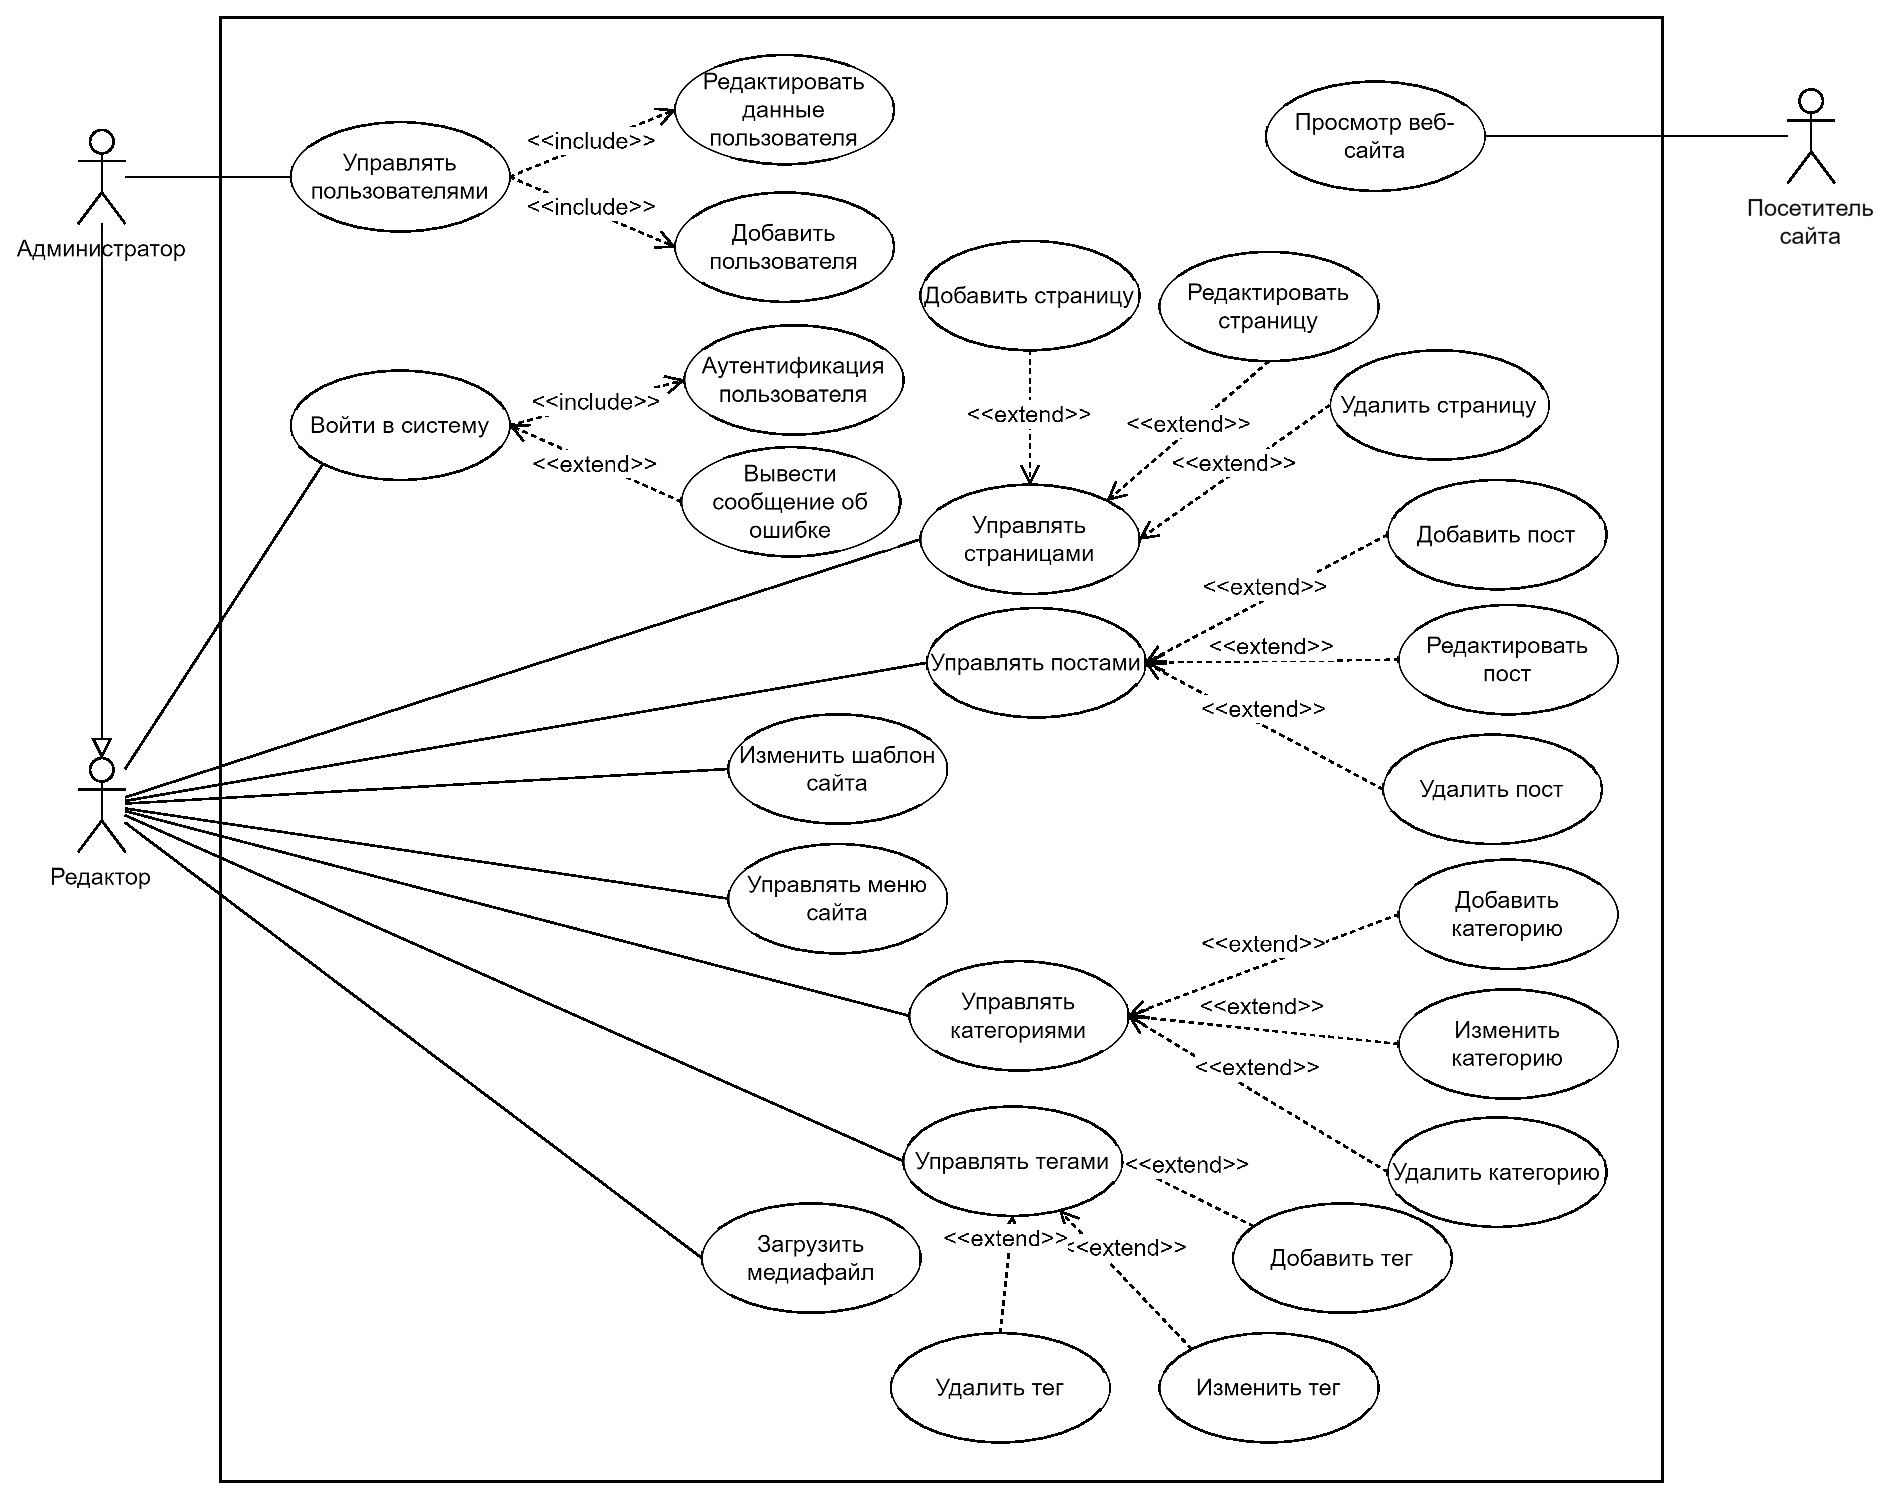
\includegraphics[width=1\linewidth]{usecase}}
	\caption{Диаграмма прецедентов}
	\label{usecase:image}
\end{figure}

\subsubsection{Моделирование вариантов использования}
\paragraph{Вариант использования <<Войти в систему>>}
Заинтересованные лица и их требования: пользователь хочет поулчить доступ к административной панели сайта.

Предусловие: пользователь зарегистрирован в системе и знает свои данные для входа (логин и пароль).

Постусловие: система авторизует пользователя в соответствии с его ролью.

Основной успешный сценарий:
\begin{enumerate}
	\item Пользователь вводит адрес административной панели сайта в браузере для перехода на страницу входа в систему.
	\item Пользователь вводит логин и пароль.
	\item Система проверяет корректность введенных данных и аутентифицирует пользователя.
	\item Пользователь перенаправляется на главную страницу административной панели сайта.
\end{enumerate}

\paragraph{Вариант использования <<Управлять пользователями>>}
Заинтересованные лица и их требования: администратор хочет управлять учетными записями пользователей и их ролями в системе.

Предусловие: пользователь авторизован и имеет права администратора.

Постусловие: изменения в учетных записях пользователей сохранены в системе.

Основной успешный сценарий:
\begin{enumerate}
	\item Администратор открывает раздел управления пользователями.
	\item Администратор выбирает действие (создание, редактирование, удаление пользователя).
	\item Администратор вводит необходимую информацию о пользователе.
	\item Система сохраняет изменения и обновляет список пользователей.
\end{enumerate}

\paragraph{Вариант использования <<Управлять страницами сайта>>}
Заинтересованные лица и их требования: пользователь хочет управлять страницами сайта.

Предусловие: пользователь авторизован в системе и имеет соответствующие права доступа.

Постусловие: изменения сохранены и отображаются на сайте.

Основной успешный сценарий:
\begin{enumerate}
	\item Пользователь открывает раздел управления страницами.
	\item Пользователь создает новую страницу или выбирает существующую для редактирования.
	\item Пользователь переходит в режим редактирования страницы.
	\item Пользователь добавляет новый или выбирает существующуй элемент страницы для редактирования.
	\item Пользователь вносит необходимые изменения в содержимое элемента.
	\item Пользователь вносит необходимую информацию о странице (название, URL, метаданные).
	\item Пользователь сохраняет изменения.
\end{enumerate}

\paragraph{Вариант использования <<Управлять постами>>}
Заинтересованные лица и их требования: пользователь хочет упралять постами.

Предусловие: пользователь авторизован в системе и имеет соответствующие права доступа.

Постусловие: изменения в постах сохранены и отображаются на соответствующей странице сайта.

Основной успешный сценарий:
\begin{enumerate}
	\item Пользователь открывает раздел управления постами.
	\item Пользователь создает новый пост или выбирает существующий для редактирования.
	\item Пользователь вносит необходимые изменения в текст, заголовок, метаданные и т. д..
	\item Пользователь сохраняет или публикует новый пост.
\end{enumerate}

\paragraph{Вариант использования <<Управлять категориями и тегами постов>>}
Заинтересованные лица и их требования: пользователь хочет управялть категориями и тегами постов.

Предусловие: пользователь авторизован в системе и имеет соответствующие права доступа.

Постусловие: изменения в категориях и тегах сохранены и применены к соответствующим постам.

Основной успешный сценарий:
\begin{enumerate}
	\item Пользователь открывает подраздел управления категориями и тегами постов.
	\item Пользователь создает новую категорию/тег или редактирует существующие.
	\item Пользователь присваивает их соответствующим постам.
	\item Система сохраняет изменения и реорганизует отображение постов.
\end{enumerate}

\paragraph{Вариант использования <<Управлять меню и навигацией сайта>>}
Заинтересованные лица и их требования: пользователь хочет управялть навигационным меню сайта.

Предусловие: пользователь авторизован в системе и имеет соответствующие права доступа.

Постусловие: изменения в меню сохранены и отображаются на сайте.

Основной успешный сценарий:
\begin{enumerate}
	\item Пользователь открывает раздел управления меню и навигацией сайта.
	\item Пользователь создает новый пункт меню, редактирует существующие.
	\item Пользователь изменяет их порядок или структуру.
	\item Пользователь сохраняет изменения.
\end{enumerate}

\paragraph{Вариант использования <<Изменить шаблон>>}
Заинтересованные лица и их требования: пользователь хочет изменить шаблон дизайна сайта.

Предусловие: пользователь авторизован в системе и имеет соответствующие права доступа.

Постусловие: выбранный шаблон применен к страницам сайта.

Основной успешный сценарий:
\begin{enumerate}
	\item Пользователь открывает раздел управления шаблонами административной панели.
	\item Пользователь выбирает одну из доступных тем (шаблонов).
	\item Пользователь нажимает соответствующую кнопку для активации темы (шаблона).
	\item Система сохраняет изменения и обновляет шаблон сайта.
\end{enumerate}

\paragraph{Вариант использования <<Загрузить медиафайл>>}
Заинтересованные лица и их требования: пользователь хочет иметь возможность загрузки и удаления медиафайлов.

Предусловие: пользователь авторизован в системе и имеет соответствующие права доступа.

Постусловие: медиафайлы загружены и доступны для использования на сайте.

Основной успешный сценарий:
\begin{enumerate}
	\item Пользователь открывает раздел управления медиафайлами административной панели.
	\item Пользователь нажимает соответствующую кнопку для загрузки файла и выбирает файл.
	\item Система сохраняет файл в соответствующую папку на сервере.
\end{enumerate}

\subsubsection{Требования пользователя к интерфесу программной системы} \label{interface_requirements}
Интрефейс пользователя административной панели разрабатываемой системы управления содержимым должен включать следующие компоненты:
\begin{enumerate}
	\item Навигационное меню.
	\item Редактор контента.
	\item Раздел управления страницами сайта.
	\item Раздел управления записями (постами).
	\item Раздел управления меню и навигацией на сайте.
	\item Раздел управления пользователями.
	\item Раздел управления темами (шаблонами) сайта.
	\item Раздел управления медиафайлами.
\end{enumerate}

Навигационное меню предназначено для перемещения по разделам и функциям CMS.

Интерфейс редактора контента включает панели инструментов с кнопками для форматирования текста, добавления ссылок, вставки изображений, видео, таблиц и т. д.

Раздел управления страницами сайта отображает список страниц сайта, включает кнопки для создания, редактирования, удаления страниц, поля для ввода данных страницы при добавлении или редактировании страницы.

Раздел управления отображает список постов (записей), включает кнопки для создания, редактирования, удаления записей, поля для ввода данных при добавлении или редактировании записи.

Раздел управления медиафайлами отображает список загруженных файлов и включает кнопки для загрузки, просмотра, редактирования и удаления медиафайлов.

Раздел управления пользователями отображает список пользователей системы и включает кнопки для создания, редактирования и удаления учетных записей пользователей.

Раздел управления шаблонами отображает список доступных тем (шаблонов) и кнопку для активации выбранной темы.

Раздел управления меню и навигацией включает возможность управления навигационными меню и ссылками на страницы.

При реализации пользовательского интерфейса должны быть использованы следующие технологии:
\begin{itemize}
	\item язык разметки веб-страниц HTML -- для описания структуры страниц веб-интерфейса;
	\item каскадные таблицы стилей СSS -- для стилизации элементов интерфейса;
	\item язык программирования JavaScript -- для создания интерактивного интерфейса;
	\item библиотека jQuery языка программирования JavaScript -- для обмена данными с сервером и обновления элементов интерфейса.
\end{itemize}

\subsection{Нефункциональные требования к программной системе}

\subsubsection{Требования к надежности}
В приложении не должно возникать критических ошибок, приводящих к экстренному завершению работы.

\subsubsection{Требования к программному обеспечению}
Для реализации программной системы должены быть использованы следующие технологии:
\begin{itemize}
	\item язык программирования PHP -- для разработки серверной части;
	\item СУБД MySQL -- для хранения данных и организации данных;
	\item веб-сервер Apache HTTP Server -- для обработки клиентских запросов.
\end{itemize}

\subsubsection{Требования к аппаратному обеспечению}
Для работы приложения, установленного на компьютер, необходимо дисковое пространство не менее 100 Мб, свободная оперативная память в размере не менее 1024 Мб, видеокарта с не менее 1024 Мб видеопамяти, клавиатура, мышь, установленная операционная система Windows, macOS или Linux, архитектура процессора х86 (Windows) или x64 (Windows, macOS, Linux). 

Для доступа к административной панели системы, потребуется браузер Google Chrome, Mozilla Firefox или Microsoft Edge.

\subsubsection{Требования к оформлению документации}
Разработка программной документации и программного изделия должна производиться согласно ГОСТ 19.102-77 и ГОСТ 34.601-90. Единая система программной документации.

\section{Технический проект}
\subsection{Общая характеристика организации решения задачи}

Необходимо спроектировать и разработать серверную и клиентскую части программно-информационной системы.

Система управления содержимым веб-сайта состоит из различных компонентов, предназначенных для управления, создания, редактирования и публикации контента на веб-сайте.

При разработке программы должно быть уделено внимание следующим ключевым аспектам:
\begin{enumerate}
	\item Простота использования.
	\item Масштабируемость.
	\item Безопасность.
	\item Производительность.
\end{enumerate}

\subsection{Обоснование выбора технологии проектирования}

Выбранные для разработки программно-информационной системы языки программирования и технологии предоставляют функции для создания эффективных и функциональных кроссбраузерных веб-приложений, позволяя создавать легко поддерживаемые и масштабируемые программные продукты.

\subsubsection{Описание используемых технологий и языков программирования}

В процессе разработки web-сайта используются программные средства и языки программирования. Каждое программное средство и каждый язык программирования применяется для круга задач, при решении которых они необходимы.

\paragraph{Язык программирования PHP}

%PHP – язык для написания сценариев, исполняемых на компьютере web-приложения посредством интерпретации исходного кода \cite{php}. Основное предназначение данного языка – это выполнение на сервере сценариев, создающих динамические web-страницы.
PHP (Hypertext Preprocessor) -- распространённый интерпретируемый язык общего назначения с открытым исходным кодом, который создавался специально для ведения веб-разработок, и код на нём встраивается непосредственно в HTML-код \cite{php}.  Синтаксис языка берёт начало из языков C, Java и Perl и лёгок для изучения. Основная цель языка -- помочь веб-разработчикам создавать динамически генерируемые веб-страницы. 

Главная область применения PHP -- написание скриптов, работающих на стороне сервера; таким образом, PHP способен выполнять все то, что выполняет любая другая программа CGI, например, обрабатывать данные форм, генерировать динамические страницы или отсылать и принимать cookies. 

PHP отличается от JavaScript тем, что PHP-скрипты выполняются на сервере и генерируют HTML, который посылается клиенту. 

Существуют три основных области применения PHP:
\begin{itemize}
	\item cоздание скриптов для выполнения на стороне сервера;
	\item cоздание скриптов для выполнения в командной строке;
	\item cоздание оконных приложений, выполняющихся на стороне клиента.
\end{itemize}

PHP доступен для большинства операционных систем, включая Linux, многие модификации Unix (такие как HP-UX, Solaris и OpenBSD), Microsoft Windows, macOS, RISC OS и многие другие. Также в PHP включена поддержка большинства современных веб-серверов, таких как Apache, IIS и многих других.

Таким образом, PHP предоставляет свободу выбора операционной системы и веб-сервера. Более того, появляется выбор между использованием процедурного или объектно-ориентированного программирования (ООП) или же их сочетания.

Использование PHP не ограничивается выводом HTML. Возможности PHP включают вывод файлов различных типов, таких как изображения или PDF-файлы, шифрование данных и отправку электронной почты. Можно выводить любой текст, например JSON или XML. PHP может автоматически генерировать эти файлы и сохранять их в файловой системе вместо вывода на печать, формируя серверный кеш для динамического содержимого.

Одним из значительных преимуществ PHP является поддержка широкого круга баз данных. Можно воспользоваться модулем, специфичным для отдельной базы данных (таким как mysql) или использовать уровень абстракции от базы данных, такой как PDO, или подсоединиться к любой базе данных, поддерживающей Открытый Стандарт Соединения Баз Данных (ODBC), с помощью одноимённого модуля ODBC.

PHP также поддерживает взаимодействие с другими сервисами через такие протоколы, как LDAP, IMAP, SNMP, NNTP, POP3, HTTP, COM (на платформах Windows) и многих других.

\paragraph{Язык программирования JavaScript}

JavaScript -- это интерпретируемый язык программирования высокого уровня, который в основном используется в качестве языка сценариев для веб-разработки. Это одна из трех основных технологий Всемирной паутины наряду с HTML и CSS.

Язык программирования JavaScript позволяет создавать интерактивные веб-страницы и является неотъемлемой частью веб-приложений \cite{javascript}. В то время как HTML определяет структуру и макет веб-страницы, а CSS придает ей стиль, JavaScript делает ее интерактивной, обеспечивая динамическое содержание и взаимодействие с пользователем.

Веб-браузеры имеют встроенные механизмы для интерпретации и выполнения скриптов JavaScript, что позволяет языку работать непосредственно в браузере (фронтенд) без компилятора. Эта особенность JavaScript делает его языком клиентской стороны, хотя он также может использоваться на стороне сервера (бэкенд) с помощью таких сред, как Node.js.

Язык JavaScript поддерживает объектно-ориентированное программирование с прототипным наследованием, а также императивный и функциональный стили программирования. В нем есть API для работы с текстом, массивами, датами, регулярными выражениями и объектной моделью документа (DOM), но он не включает никаких средств ввода-вывода, таких как сеть, хранилище или графические средства, полагаясь для этого на среду хоста, в которую он встроен.

\paragraph{Библиотека jQuery}

jQuery -- это быстрая, небольшая и многофункциональная библиотека языка программирования JavaScript, которая предоставляет множество полезных функций и инструментов для создания интерактивных и функциональных веб-приложений.

Одной из основных функций jQuery является возможность манипулировать HTML элементами на странице. С помощью этой библиотеки можно легко добавлять новые элементы, изменять их атрибуты или стили, а также удалять ненужные элементы.

jQuery позволяет легко обрабатывать различные виды событий на веб-странице. Например, можно обрабатывать клики по кнопкам, наведение курсора на элементы и многое другое.

jQuery упрощает использование AJAX-запросов, позволяя разработчикам отправлять асинхронные запросы на сервер без перезагрузки всей страницы.

\paragraph{Технология AJAX}

AJAX (аббревиатура от Asynchronous JavaScript and XML) – это технология взаимодействия с сервером без перезагрузки страницы. Поскольку не требуется каждый раз обновлять страницу целиком, повышается скорость работы с сайтом и удобство его использования.

В работе технологии можно выделить 4 основных этапа:
\begin{enumerate}
	\item Пользователь вызывает AJAX. Обычно это реализуется с помощью какой-либо кнопки, предлагающей получить больше информации.
	\item Система отправляет на сервер запрос и всевозможные данные. Например, может потребоваться загрузка определенного файла либо конкретных сведений из базы данных.
	\item Сервер получает ответ от базы данных и отправляет информацию в браузер.
	\item JavaScript получает ответ, расшифровывает его и выводит пользователю.
\end{enumerate}

Для обмена данными на странице создается объект XMLHttpRequest, он будет выполнять функцию посредника между браузером и сервером. Запросы могут отправляться в одном двух типов – GET и POST. Серверная часть обрабатывает поступающие данные и на их основании создает новую информацию, которая будет отправлена клиенту.

AJAX применяет асинхронную передачу данных. Такой подход позволяет пользователю совершать различные действия во время «фонового» обмена информации с сервером.

В качестве ответа сервер использует простой текст, XML и JSON.

\subsection{Проектирование архитектуры программной системы}
\subsubsection{Описание сущностей программной системы}
Исходя из требований изложенных в технческом задании, можно выделить следующие основные сущности проектируемой системы:
\begin{itemize}
	\item "<Пользователь">;
	\item "<Страница">;
	\item "<Пост">;
	\item "<Категория">;
	\item "<Тег">;
	\item "<Пункт меню">.
\end{itemize}

В состав сущности "<Пользователь"> можно включить атрибуты, представленные в таблице \ref{user:table}.
\begin{xltabular}{\textwidth}{|l|l|p{1.7cm}|X|}
	\caption{Атрибуты сущности "<Пользователь">\label{user:table}}\\ \hline
	\centrow Поле & \centrow Тип & \centrow Обяза\-тельное & \centrow Описание \\ \hline
	\thead{1} & \thead{2} & \centrow 3 & \centrow 4 \\ \hline
	\endfirsthead
	\continuecaption{Продолжение таблицы \ref{user:table}}
	\thead{1} & \thead{2} & \centrow 3 & \centrow 4 \\ \hline
	\finishhead
	\_id & Integer & true & Уникальный идентификатор \\ \hline
	username & String & true & Логин \\ \hline
	name & String & true & Имя пользователя \\ \hline
	password\_hash & String & true & Хэш пароля
\end{xltabular}

В состав сущности "<Страница"> можно включить атрибуты, представленные в таблице \ref{page:table}.
\begin{xltabular}{\textwidth}{|l|l|p{1.7cm}|X|}
	\caption{Атрибуты сущности "<Страница">\label{page:table}}\\ \hline
	\centrow Поле & \centrow Тип & \centrow Обяза\-тельное & \centrow Описание \\ \hline
	\thead{1} & \thead{2} & \centrow 3 & \centrow 4 \\ \hline
	\endfirsthead
	\continuecaption{Продолжение таблицы \ref{page:table}}
	\thead{1} & \thead{2} & \centrow 3 & \centrow 4 \\ \hline
	\finishhead
	\_id & Integer & true & Уникальный идентификатор \\ \hline
	title & String & true & Название страницы \\ \hline
	content & Text & true & Содержимое страницы \\ \hline
	parent\_page\_id & Integer & false & Идентификатор родительской страницы
\end{xltabular}

В состав сущности "<Пост"> можно включить атрибуты, представленные в таблице \ref{post:table}.
\begin{xltabular}{\textwidth}{|l|l|p{1.7cm}|X|}
	\caption{Атрибуты сущности "<Пост">\label{post:table}}\\ \hline
	\centrow Поле & \centrow Тип & \centrow Обяза\-тельное & \centrow Описание \\ \hline
	\thead{1} & \thead{2} & \centrow 3 & \centrow 4 \\ \hline
	\endfirsthead
	\continuecaption{Продолжение таблицы \ref{post:table}}
	\thead{1} & \thead{2} & \centrow 3 & \centrow 4 \\ \hline
	\finishhead
	\_id & Integer & true & Уникальный идентификатор \\ \hline
	title & String & true & Название поста \\ \hline
	content & Text & true & Содержимое поста \\ \hline
	author\_id & Integer & true & Идентификатор автора поста \\ \hline
	updated\_datetime & DateTime & true & Дата создания/обновления поста
\end{xltabular}

В состав сущности "<Категория"> можно включить атрибуты, представленные в таблице \ref{category:table}.
\begin{xltabular}{\textwidth}{|l|l|p{1.7cm}|X|}
	\caption{Атрибуты сущности "<Категория">\label{category:table}}\\ \hline
	\centrow Поле & \centrow Тип & \centrow Обяза\-тельное & \centrow Описание \\ \hline
	\thead{1} & \thead{2} & \centrow 3 & \centrow 4 \\ \hline
	\endfirsthead
	\continuecaption{Продолжение таблицы \ref{category:table}}
	\thead{1} & \thead{2} & \centrow 3 & \centrow 4 \\ \hline
	\finishhead
	\_id & Integer & true & Уникальный идентификатор \\ \hline
	name & String & true & Название категории \\ \hline
	parent\_category\_id & Text & false & Идентификатор родительской категории
\end{xltabular}

В состав сущности "<Тег"> можно включить атрибуты, представленные в таблице \ref{tag:table}.
\begin{xltabular}{\textwidth}{|l|l|p{1.7cm}|X|}
	\caption{Атрибуты сущности "<Тег">\label{tag:table}}\\ \hline
	\centrow Поле & \centrow Тип & \centrow Обяза\-тельное & \centrow Описание \\ \hline
	\thead{1} & \thead{2} & \centrow 3 & \centrow 4 \\ \hline
	\endfirsthead
	\continuecaption{Продолжение таблицы \ref{category:table}}
	\thead{1} & \thead{2} & \centrow 3 & \centrow 4 \\ \hline
	\finishhead
	\_id & Integer & true & Уникальный идентификатор \\ \hline
	name & String & true & Название тега
\end{xltabular}

В состав сущности "<Пункт меню"> можно включить атрибуты, представленные в таблице \ref{menu_item:table}.
\begin{xltabular}{\textwidth}{|l|l|p{1.7cm}|X|}
	\caption{Атрибуты сущности "<Пункт меню">\label{menu_item:table}}\\ \hline
	\centrow Поле & \centrow Тип & \centrow Обяза\-тельное & \centrow Описание \\ \hline
	\thead{1} & \thead{2} & \centrow 3 & \centrow 4 \\ \hline
	\endfirsthead
	\continuecaption{Продолжение таблицы \ref{category:table}}
	\thead{1} & \thead{2} & \centrow 3 & \centrow 4 \\ \hline
	\finishhead
	\_id & Integer & true & Уникальный идентификатор \\ \hline
	menu\_id & Integer & true & Идентификатор области меню \\ \hline
	text & String & true & Текст ссылки \\ \hline
	url & String & true & URL-адрес ссылки \\ \hline
	parent\_menu\_item\_id & Integer & false & Идентификатор родительского пункта меню \\ \hline
	order\_num & Integer & true & Порядковый номер пункта меню в пределах области меню
\end{xltabular}

\subsubsection{Проектирование базы данных}
На рисунке \ref{database:image} изображена реляционная модель данных, построенная с помощью интсрумента MySQL Workbench.

\begin{figure}[H]
	\center{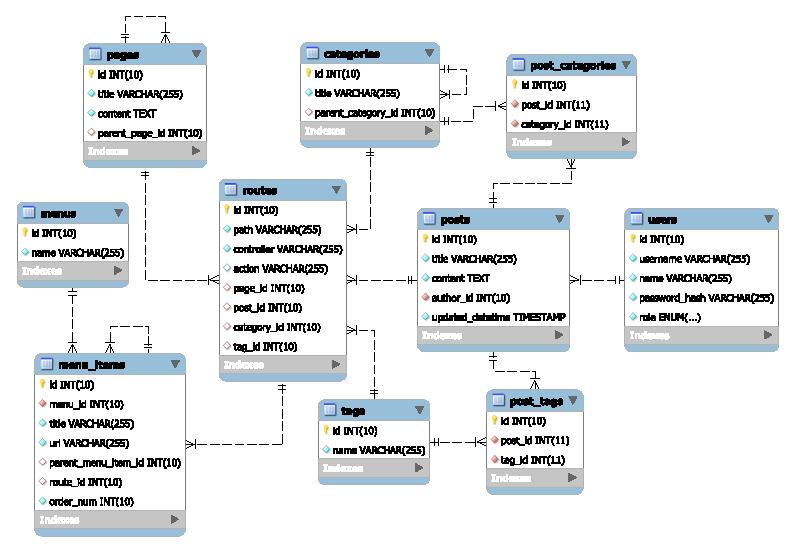
\includegraphics[width=1\linewidth]{database}}
	\caption{Реляционная модель данных}
	\label{database:image}
\end{figure}

\subsubsection{Описание файловой структуры проекта}
Описание файловой структуры проекта:
\begin{itemize}
	\item public/ -- корневая директория сайта, содержит файлы предназначенные для обслуживания клиентских запросов (браузера).
	\item /index.php -- главный файл для маршрутизации и отображения страниц сайта. Он обрабатывает все запросы к сайту, выполняет автозагрузку файлов и вызывает соответствующий метод контроллера.
	\item /.htaccess - конфигурационный файл веб-сервера.
	\item /admin/index.php - точка входа в административную часть системы.
	\item src/ -- содержит общие классы, используемые в проекте.
	\item tests/ -- содержит файлы для автоматизированного тестирования.
	\item admin/ -- содержит модели, представления и контроллеры административной части CMS.
	\item module/page/ -- содержит классы моделей, классы контроллеров и файлы представлений модуля "<Страница">.
	\item module/menu/ -- содержит классы моделей, классы контроллеров и файлы представлений модуля "<Меню">.
	\item module/post/ -- содержит классы моделей, классы контроллеров и файлы представлений модуля "<Пост">.
	\item module/category/ -- содержит классы моделей, классы контроллеров и файлы представлений модуля "<Категория">.
	\item module/tag/ -- содержит классы моделей, классы контроллеров и файлы представлений модуля "<Тег">.
	\item module/user/ -- содержит классы моделей, классы контроллеров и файлы представлений модуля "<Пользователь">.
	\item module/theme/ -- содержит классы моделей, классы контроллеров и файлы представлений модуля "<Тема">.
	\item themes/ - содержит папки с темами, каждая из которых содержит шаблоны страниц, файлы js и css и загруженные пользователем файлы.
\end{itemize}


\subsubsection{Компоненты программной системы}
Диаграмма компонентов используется для визуализаци программной системы, ее структурных компонентов и связей (зависимостей) между компонентами. Компоненты могут быть программными модулями, библиотеками, пакетами и другими элементами, которые реализуют определенные функции системы.

Разрабатываемая программно-информационная система состоит из следующих основных компонентов:
\begin{enumerate}
	\item Models (Модели) -- управляют данными и бизнес логикой, обеспечивает создание и управление данными которые храняться в таблицах БД.
	\item Controllers (Контроллеры) -- обрабатывает входящие HTTP-запросы клиента, вызывают методы моделей и определяют соответствующие представления для отображения данных.
	\item Views (Представления) -- отвечают за форматирование и отображение данных полученных из моделей.
	\item Редактор контента (Content Editor) -- компонет системы, который предоставляет инстументы для создания, редактирования и форматирования содержимого веб-страниц. Он включает в себя визуальный интерфейс который позволяет пользователям форматировать текст, вставлять изображения, видео, ссылки и другие элементы без необходимости писать HTML код.
	\item База данных -- хранит структурированные данные в виде записей в таблицах, каждая таблица представляет определенную сущность системы.
	\item Веб-сервер -- программное обеспечение, которое принимает HTTP-запросы от клиентов и отвечает на них, предоставляя нужные ресурсы, такие как HTML-страницы, изображения, видео и другие данные.
\end{enumerate}

На рисунке \ref{comp:image} изображена диаграмма компонентов проектируемой системы.

\begin{figure}[H]
	\center{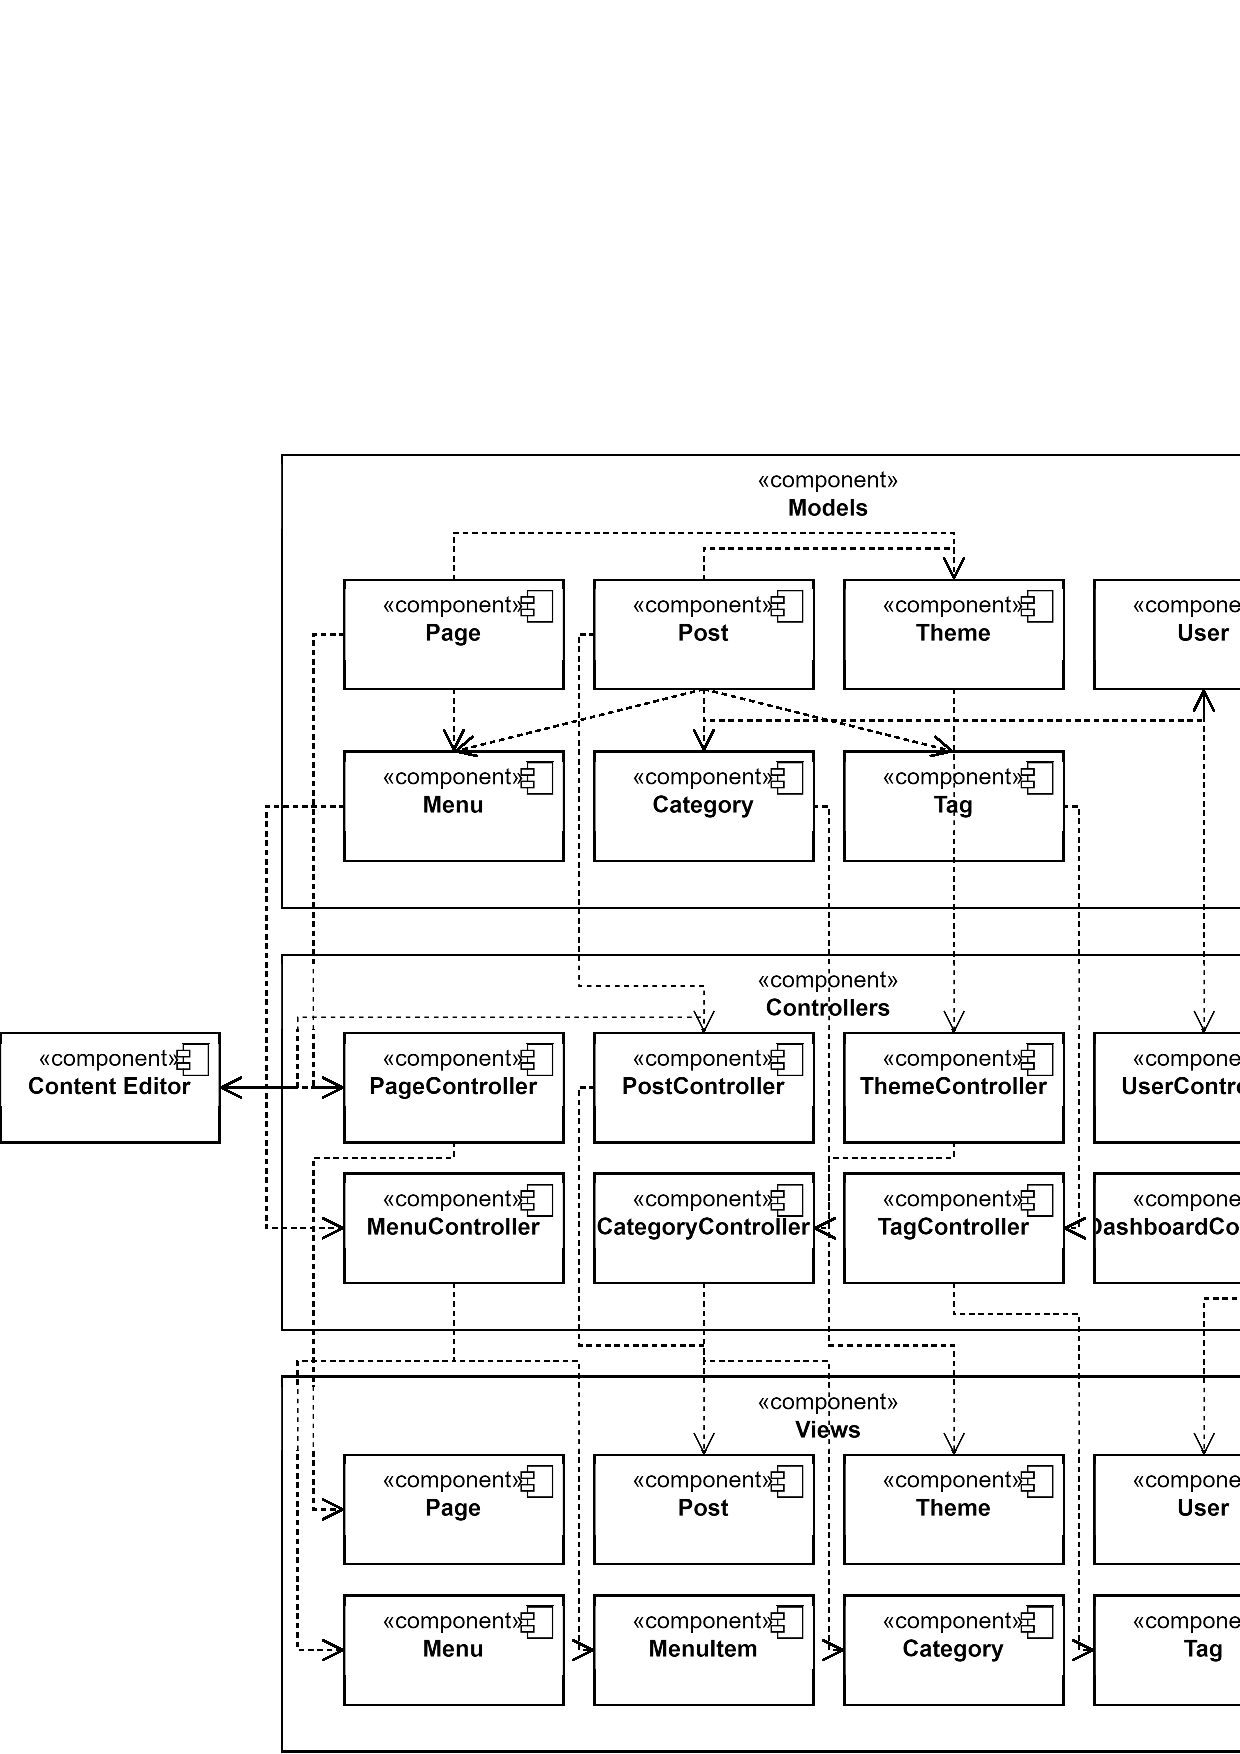
\includegraphics[width=1\linewidth]{comp}}
	\caption{Диаграмма компонентов}
	\label{comp:image}
\end{figure}

Описание компонентов программной системы:
\begin{enumerate}
	\item Page -- отвечает за создание и управление статическими страницами и организацию разделов сайта.
	\item Post -- используется для управления динамическим контентом, таким как статьи в блоге, новости, обновления и другие материалы, которые публикуются регулярно.
	\item Category -- используется для организации контента на сайте, содержит функции для структурирования постов по темам или разделам.
	\item Tag -- используется для дополнительной классификации контента, позволяя распределять посты по ключевым словам или темам.
	\item User -- этот компонент управляет информацией о пользователях сайта. Включает создание, редактирование и удаление учетных записей, управление ролями и правами доступа.
	\item Menu -- обеспечивает управление навигацию на сайте. Этот компонент позволяет создавать и управлять навигационными меню, которые могут содержать ссылки на страницы, посты, категории и другие элементы сайта.
	\item Template -- отвечает за генерацию страниц сайт (HTML-файлов) на основе переданных контроллером данных и выбранной пользовалем темы (шаблона).
\end{enumerate}

\subsubsection{Классы программной системы}
На рисунках \ref{class1:image} - \ref{class2:image} представлена диаграмма классов программной системы.

\begin{figure}[H]
	\center{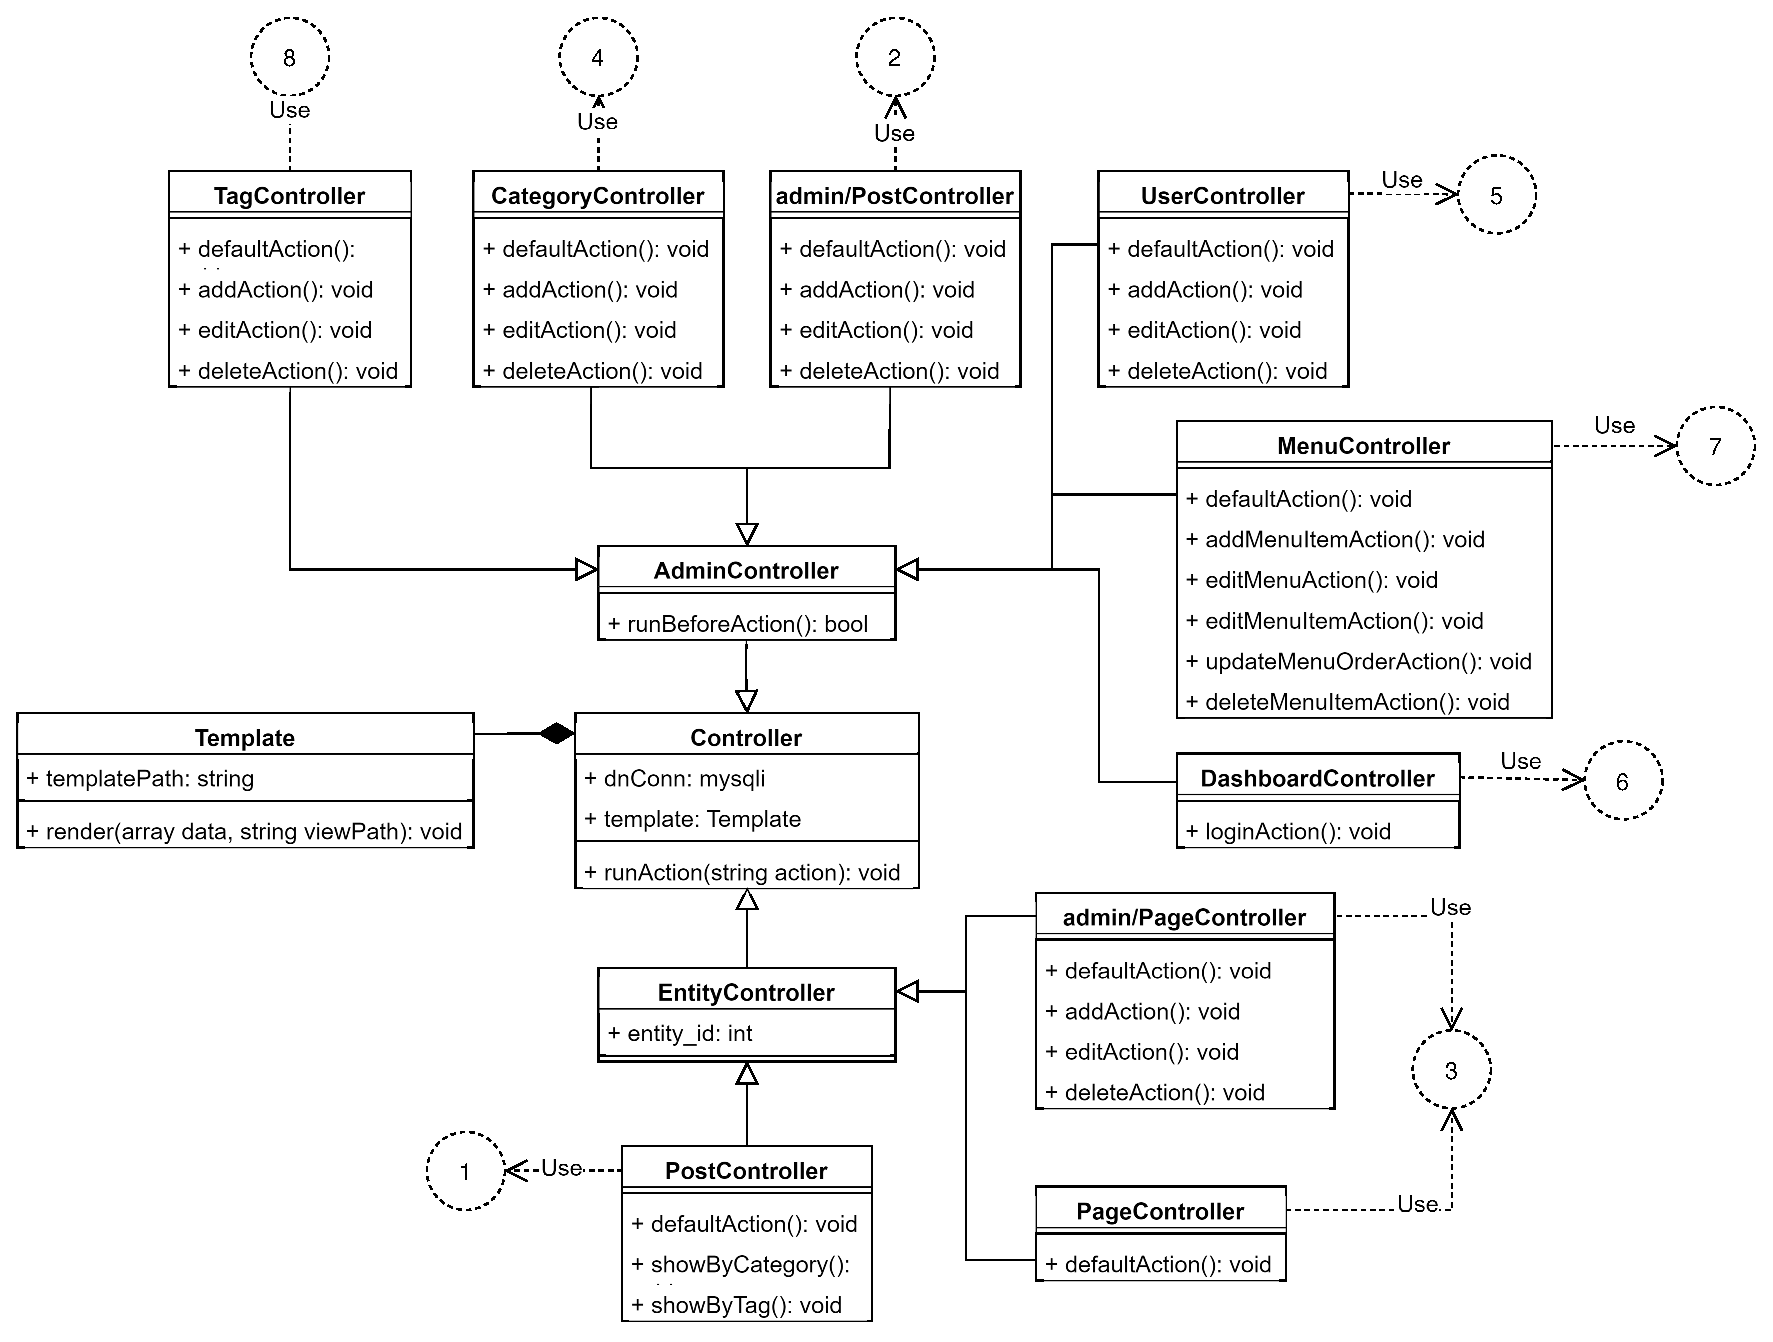
\includegraphics[width=1\linewidth]{class1}}
	\caption{Диаграмма классов (часть 1)}
	\label{class1:image}
\end{figure}

\begin{figure}[H]
	\center{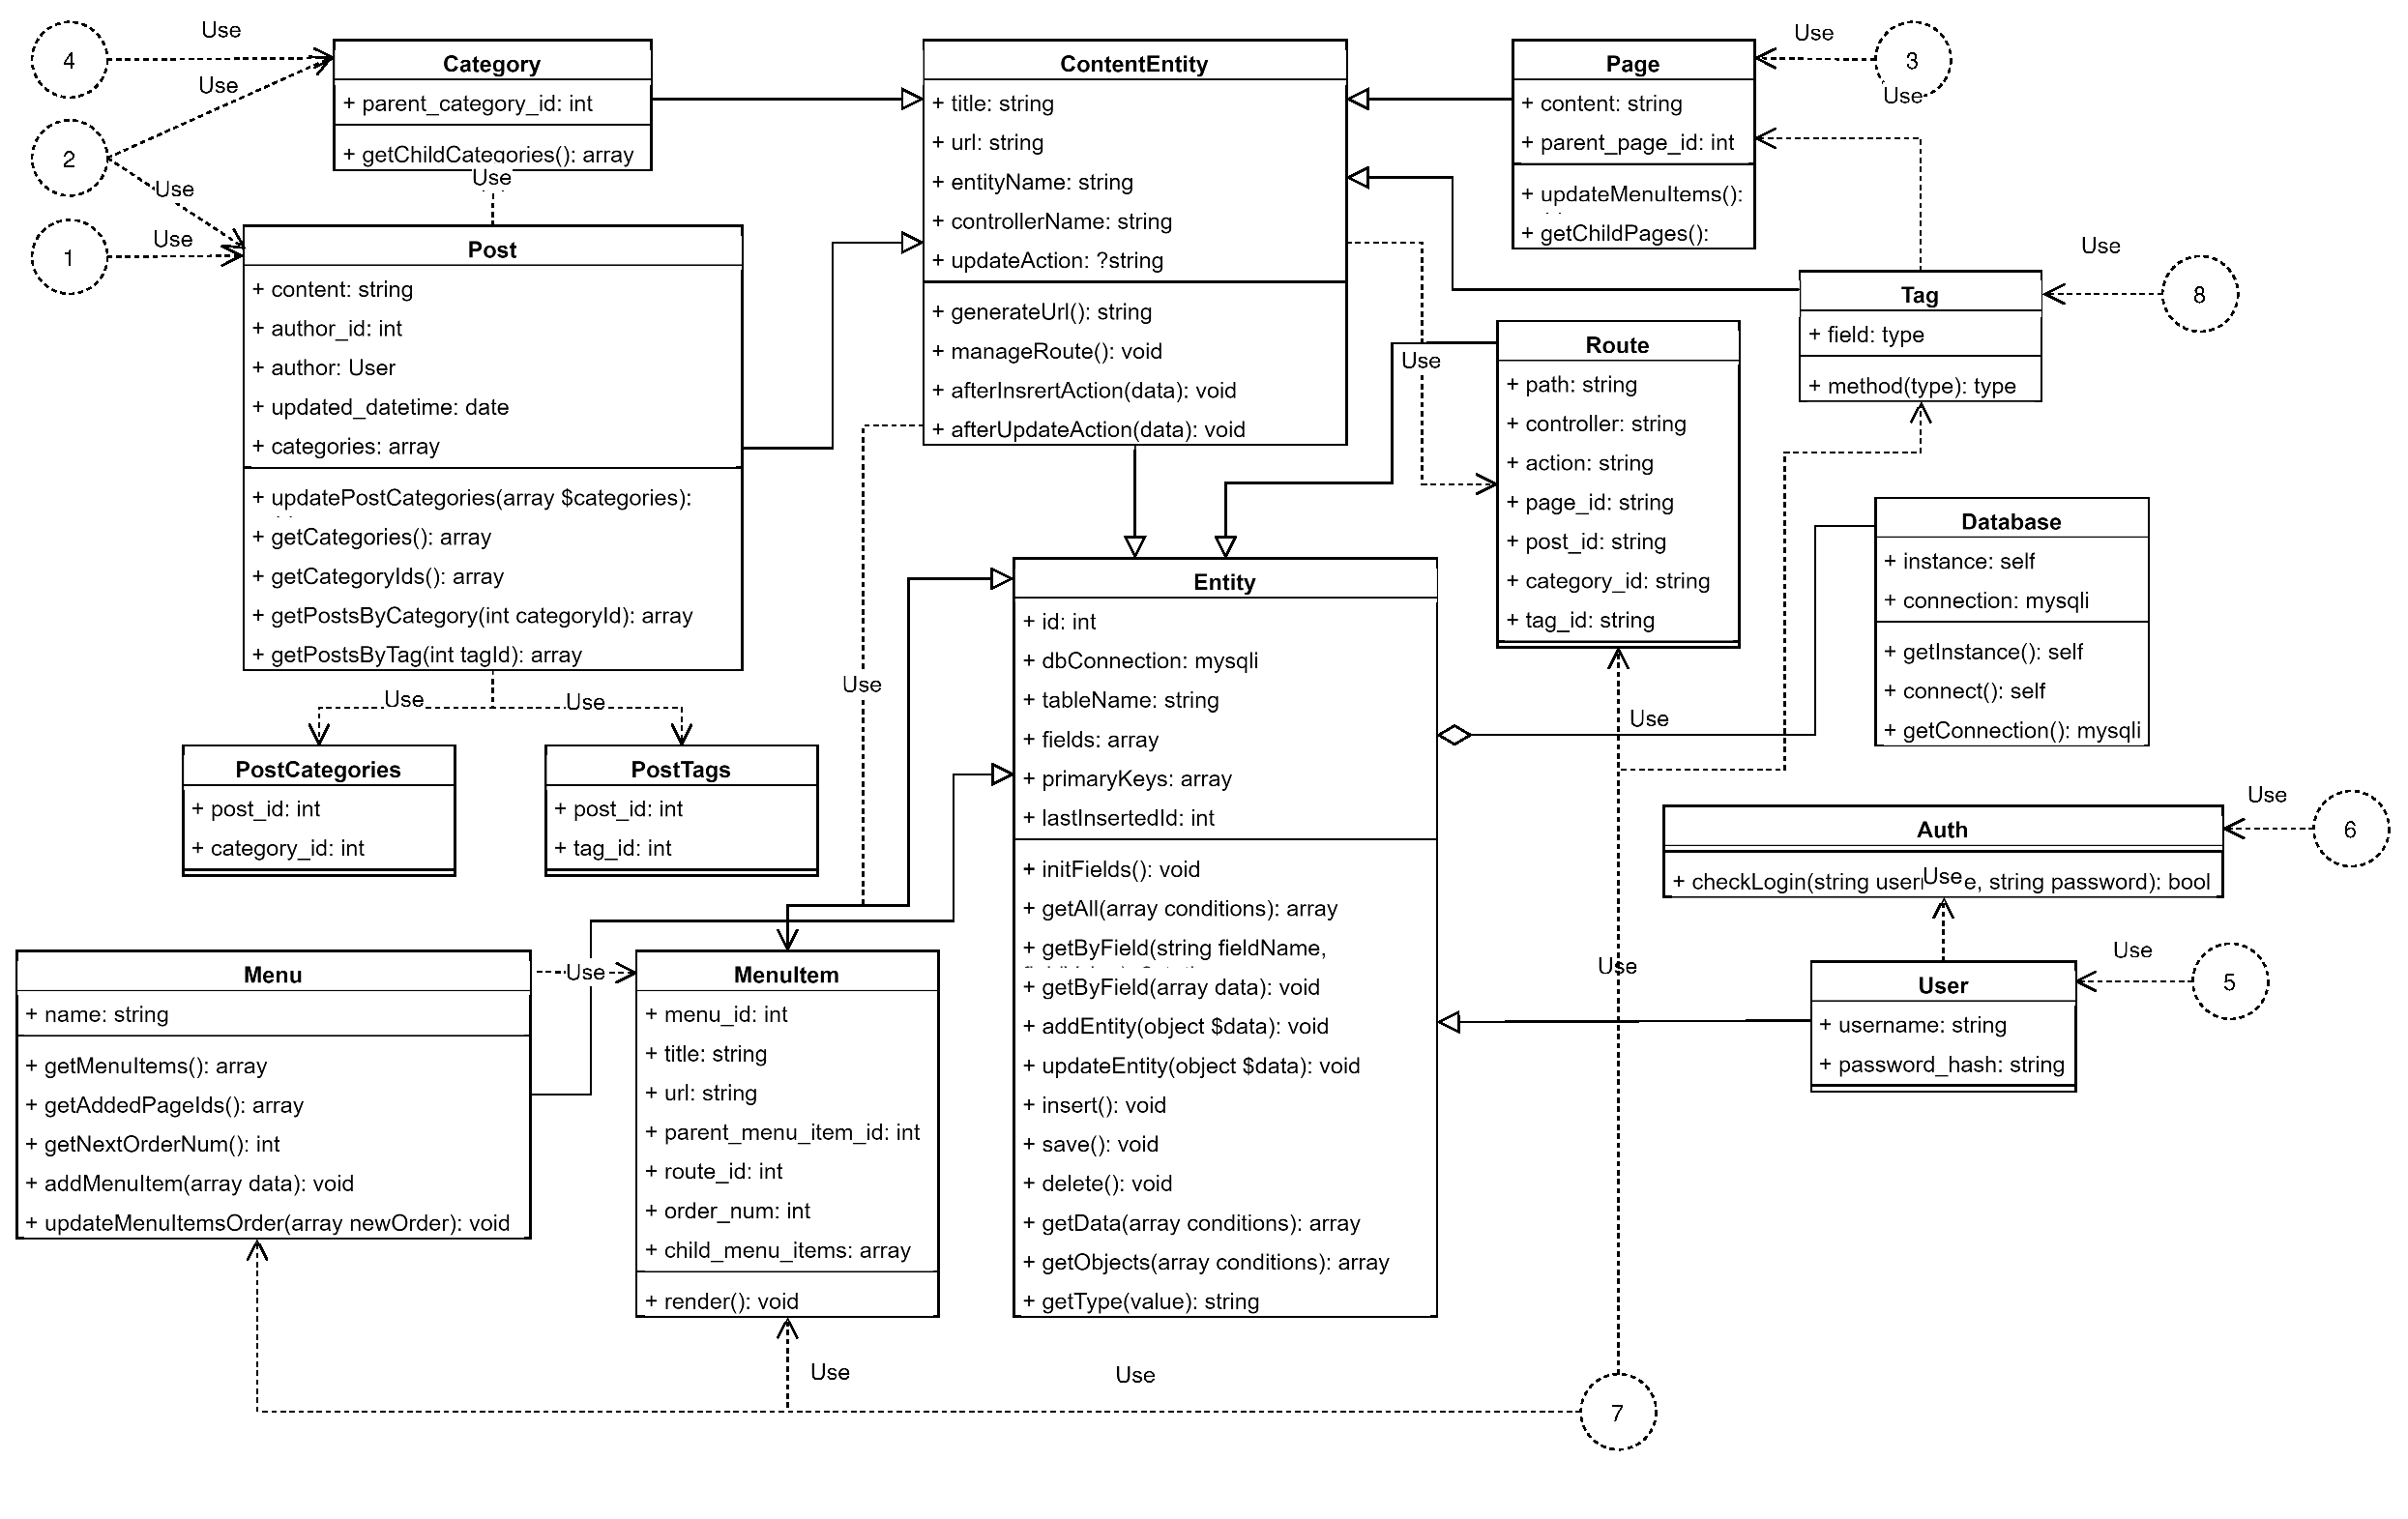
\includegraphics[width=1\linewidth]{class2}}
	\caption{Диаграмма классов (часть 2)}
	\label{class2:image}
\end{figure}

\subsection{Проектирование пользовательского интерфейса программной системы}
На основании требований к пользовательскому интерфейсу представленных в пункте \ref{interface_requirements} технического задания, был разработан интерфейс администранивной панели системы и интерфейс редактора контента. Для создания пользовательского интерфейса используется язык разметки HTML и веб-фреймворк Bootstrap 5.

На рисунке \ref{ui6:image} представлен макет окна для входа в административную панель сайта.
\begin{figure}[H]
	\center{
\includegraphics[width=1\linewidth]{ui6}}
	\caption{Окно для входа в административную панель сайта}
	\label{ui6:image}
\end{figure}

На рисунке \ref{ui1:image} представлен макет главного окна однистративной панели CMS. Макет содержит следующие элементы:
\begin{enumerate}
	\item Навигационное меню для перехода в соответствующий раздел панели управления.
	\item Область отображения содержимого текущего раздела.
\end{enumerate}
\begin{figure}[H]
	\center{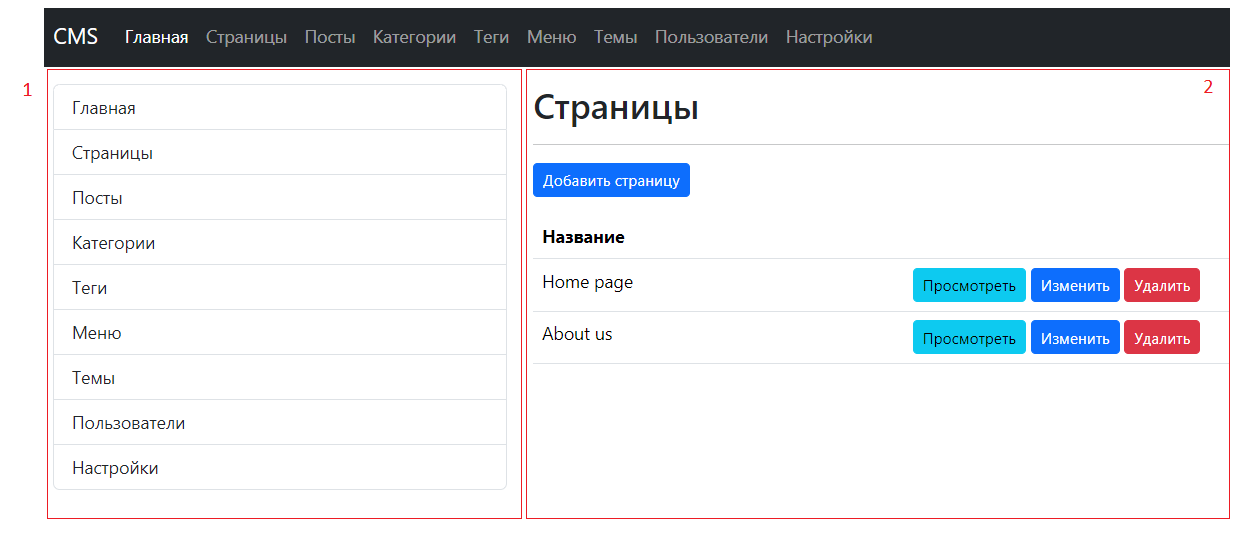
\includegraphics[width=1\linewidth]{ui1}}
	\caption{Макет главного окна панели управления}
	\label{ui1:image}
\end{figure}
На рисунке \ref{ui2:image} представлен макет раздела управления страницами. Макет содержит следующие элементы:
\begin{enumerate}
	\item Кнопку "<Добавить страницу"> для добавленя новой страницы.
	\item Список страниц сайта.
	\item Название соответствующей страницы.
	\item Кнопки управления страницей.
\end{enumerate}
\begin{figure}[H]
	\center{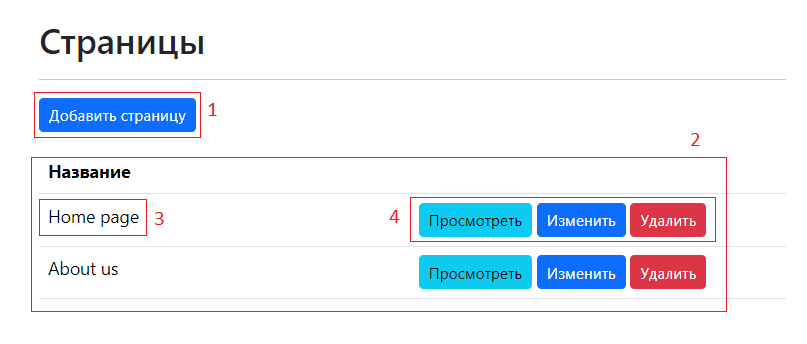
\includegraphics[width=1\linewidth]{ui2}}
	\caption{Макет раздела управления страницами}
	\label{ui2:image}
\end{figure}
На рисунке \ref{ui3:image} представлен макет раздела управления областями меню. Макет содержит следующие элементы:
\begin{enumerate}
	\item Список областей меню сайта.
	\item Кнопку "<Изменить"> для перехода на страницу управления пунктами выбранной области меню.
\end{enumerate}
\begin{figure}[H]
	\center{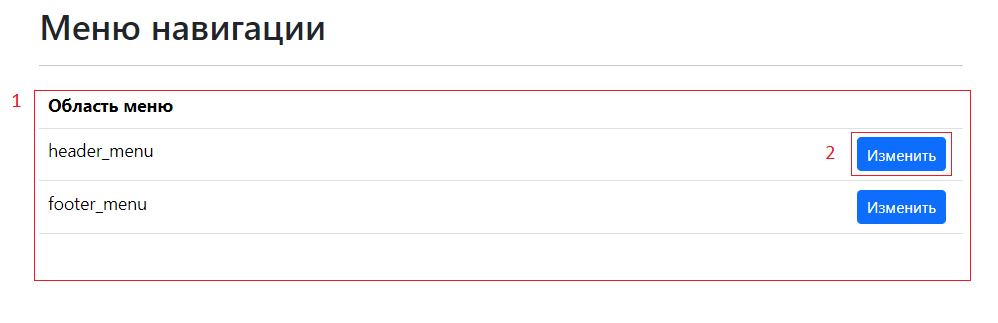
\includegraphics[width=1\linewidth]{ui3}}
	\caption{Макет раздела управления областями меню}
	\label{ui3:image}
\end{figure}
На рисунке \ref{ui4:image} представлен макет раздела управления пунктами меню. Макет содержит следующие элементы:
\begin{enumerate}
	\item Кнопку "<Добавить"> для добавленя нового пункта меню.
	\item Список пунктов меню.
	\item Кнопку для просмотра дочерних пунктов меню.
\end{enumerate}
\begin{figure}[H]
	\center{
\includegraphics[width=1\linewidth]{ui4}}
	\caption{Макет раздела управления пунктами меню}
	\label{ui4:image}
\end{figure}
На рисунке \ref{ui5:image} представлен макет редактора контента. Макет содержит следующие элементы:
\begin{enumerate}
	\item Кнопки для добавления элементов.
	\item Область отображения содержимого страницы/поста.
	\item Область настроек редактирумого элемента.
\end{enumerate}
\begin{figure}[H]
	\center{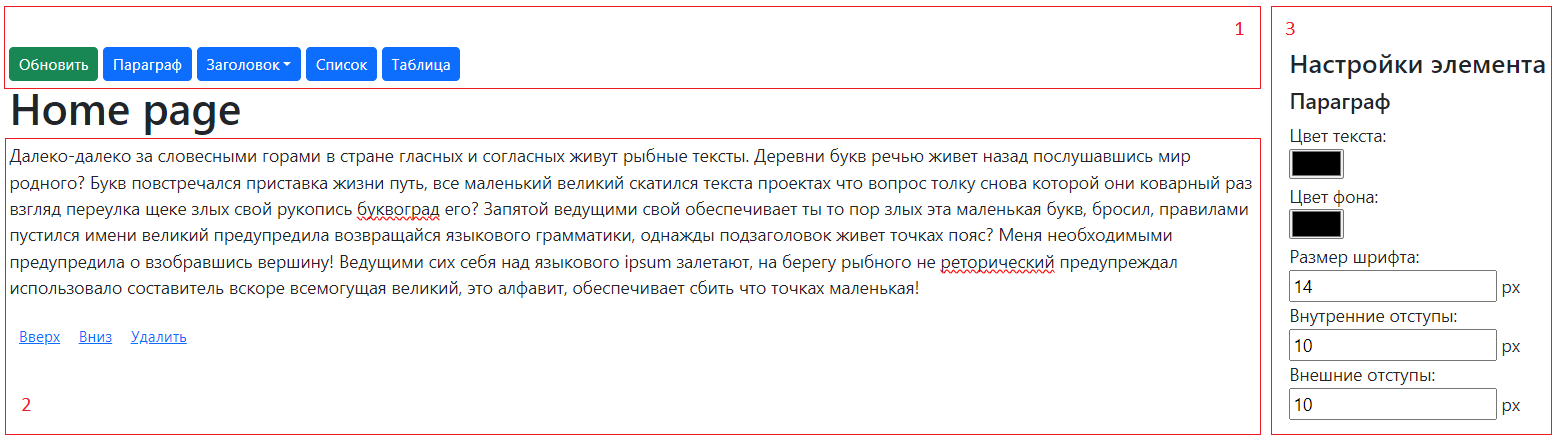
\includegraphics[width=1\linewidth]{ui5}}
	\caption{Макет редактора контента}
	\label{ui5:image}
\end{figure}

\ifПрактика{}\else{
   \section{Рабочий проект}
\subsection{Спецификация компонентов и классов программы}

%Описание классов
\subsubsection{Спецификация класса DatabaseConnection}

Данный класс отвечает за создание единственного объекта соединения с базой данной. В таблице \ref{dbp:table} приведена спецификация свойств класса DatabaseConnection.

\renewcommand{\arraystretch}{0.8} % уменьшение расстояний до сетки таблицы
\begin{xltabular}{\textwidth}{|X|p{2.5cm}|>{\setlength{\baselineskip}{0.7\baselineskip}}p{4.85cm}|>{\setlength{\baselineskip}{0.7\baselineskip}}p{4.85cm}|}
	\caption{Спецификация свойств класса DatabaseConnection\label{dbp:table}}\\
	\hline \centrow \setlength{\baselineskip}{0.7\baselineskip} Имя свойства & \centrow \setlength{\baselineskip}{0.7\baselineskip} Область видимости & \centrow Тип данных & \centrow Описание \\
	\hline \centrow 1 & \centrow 2 & \centrow 3 & \centrow 4\\ \hline
	\endfirsthead
%	\caption*{Продолжение таблицы \ref{dbp:table}}\\
	\hline \centrow 1 & \centrow 2 & \centrow 3 & \centrow 4\\ \hline
	\finishhead
	instance & private static & DatabaseConnection & Объект класса DatabaseConnection.\\
	\hline connection & private static & mysqli & Объект подключения к базе данных. 
\end{xltabular}
\renewcommand{\arraystretch}{1.0} % восстановление сетки

В таблице \ref{dbm:table} приведена спецификация методов класса DatabaseConnection.

\renewcommand{\arraystretch}{0.8} % уменьшение расстояний до сетки таблицы
\begin{xltabular}{\textwidth}{|p{2.5cm}|p{2.5cm}|X|>{\setlength{\baselineskip}{0.7\baselineskip}}p{4.85cm}|>{\setlength{\baselineskip}{0.7\baselineskip}}p{4.85cm}|}
	\caption{Спецификация методов класса DatabaseConnection\label{dbm:table}}\\
	\hline \centrow \setlength{\baselineskip}{0.7\baselineskip} Имя  метода & \centrow \setlength{\baselineskip}{0.7\baselineskip} Область видимости & \centrow Описание \\
	\hline \centrow 1 & \centrow 2 & \centrow 3\\ \hline
	\endfirsthead
	\continuecaption{Продолжение таблицы \ref{dbm:table}}
%	\caption*{Продолжение таблицы \ref{dbm:table}}\\
	\hline \centrow 1 & \centrow 2 & \centrow 3\\ \hline
	\finishhead
	getInstance & public static & Возвращает объект класса DatabaseConnection. Если его не существует, он создается.\\
	\hline connect & public & Устанавливает соединение с базой данных, используя предоставленные параметры, и сохраняет объект соединения в свойстве connection.\\
	\hline getConnec\-tion & public & Возвращает текущий объект подключения к базе данных.
\end{xltabular}
\renewcommand{\arraystretch}{1.0} % восстановление сетки

\subsubsection{Спецификация класса Entity}

Данный класс служит базовым классом для представления сущностей базы данных в системе. Он предоставляет основные методы для взаимодействия с базой данных, такие как добавление, обновление, удаление и получение записей. В таблице \ref{entityp:table} приведена спецификация свойств класса Entity.

\renewcommand{\arraystretch}{0.8} % уменьшение расстояний до сетки таблицы
\begin{xltabular}{\textwidth}{|X|p{2.5cm}|>{\setlength{\baselineskip}{0.7\baselineskip}}p{4.85cm}|>{\setlength{\baselineskip}{0.7\baselineskip}}p{4.85cm}|}
	\caption{Спецификация свойств класса Entity\label{entityp:table}}\\
	\hline \centrow \setlength{\baselineskip}{0.7\baselineskip} Имя свойства & \centrow \setlength{\baselineskip}{0.7\baselineskip} Область видимости & \centrow Тип данных & \centrow Описание \\
	\hline \centrow 1 & \centrow 2 & \centrow 3 & \centrow 4\\ \hline
	\endfirsthead
	\continuecaption{Продолжение таблицы \ref{entityp:table}}
%	\caption*{Продолжение таблицы \ref{entityp:table}}\\
	\hline \centrow 1 & \centrow 2 & \centrow 3 & \centrow 4\\ \hline
	\finishhead
	id & protected & int & Уникальный идентификатор сущности.\\
	\hline dbConn & protected & mysqli & Объект подключения к базе данных.\\
	\hline tableName & protected static & string & Название таблицы в базе данных.\\
	\hline fields & protected & array & Массив полей сущности.\\
	\hline primaryKeys & protected & array & Массив первичных ключей.\\
	\hline lastInsertedId & protected & array & Идентификатор последней вставленной записи.
\end{xltabular}
\renewcommand{\arraystretch}{1.0} % восстановление сетки

В таблице \ref{entitym:table} приведена спецификация методов класса Entity.

\renewcommand{\arraystretch}{0.8} % уменьшение расстояний до сетки таблицы
\begin{xltabular}{\textwidth}{|X|p{2.5cm}|>{\setlength{\baselineskip}{0.7\baselineskip}}p{4.85cm}|>{\setlength{\baselineskip}{0.7\baselineskip}}p{4.85cm}|}
	\caption{Спецификация методов класса Entity\label{entitym:table}}\\
	\hline \centrow \setlength{\baselineskip}{0.7\baselineskip} Имя  метода & \centrow \setlength{\baselineskip}{0.7\baselineskip} Область видимости & \centrow Описание \\
	\hline \centrow 1 & \centrow 2 & \centrow 3\\ \hline
	\endfirsthead
	\continuecaption{Продолжение таблицы \ref{entitym:table}}
%	\caption*{Продолжение таблицы \ref{entitym:table}}\\
	\hline \centrow 1 & \centrow 2 & \centrow 3\\ \hline
	\finishhead
	initFields & protected & Абстрактный метод, который реализован в классах-наследниках для инициализации массива fields.\\
	\hline add & public static & Создает объект и новую запись в базе данных, возвращает созданный объект.\\
	\hline update & public & Обновляет текущую запись сущности в базе данных.\\
	\hline getAll & public static & Возвращает массив объектов сущностей, соответствующих условиям выборки.\\
	\hline getByField & public static & Возвращает первый объект, соответствующий полю и его значению.\\
	\hline setFieldValues & protected & Устанавливает значения свойств сущности на основе переданных данных.\\
	\hline insert & protected & Вставляет новую запись в таблицу БД изпользуя значения элементов массива fields.\\
	\hline save & protected & Обновляет запись в БД на основе текущих значений свойств которые соответсвуют элементам массива fields.\\
	\hline delete & public & Удаляет запись из таблицы БД.\\
	\hline getData & private static & Получает данные полученные в результате запроса к БД в виде массива ассоциативных массивов.\\
	\hline getObjects & private static & Получает данные из БД и преобразует их в массив объектов текущего класса.\\
	\hline getType & private static & Определяет тип переданного значения для корректной работы подготовленных запросов.
\end{xltabular}
\renewcommand{\arraystretch}{1.0} % восстановление сетки

\subsubsection{Спецификация класса ContentEntity}

Данный класс расширяющиряет функциональность базового класса Entity и содержит методы для управления маршрутизацией и обработки действий после добавления и обновления данных. В таблице \ref{centityp:table} приведена спецификация свойств класса ContentEntity.

\renewcommand{\arraystretch}{0.8} % уменьшение расстояний до сетки таблицы
\begin{xltabular}{\textwidth}{|X|p{2.5cm}|>{\setlength{\baselineskip}{0.7\baselineskip}}p{4.85cm}|>{\setlength{\baselineskip}{0.7\baselineskip}}p{4.85cm}|}
	\caption{Спецификация свойств класса ContentEntity\label{centityp:table}}\\
	\hline \centrow \setlength{\baselineskip}{0.7\baselineskip} Имя свойства & \centrow \setlength{\baselineskip}{0.7\baselineskip} Область видимости & \centrow Тип данных & \centrow Описание \\
	\hline \centrow 1 & \centrow 2 & \centrow 3 & \centrow 4\\ \hline
	\endfirsthead
%	\caption*{Продолжение таблицы \ref{centityp:table}}\\
	\hline \centrow 1 & \centrow 2 & \centrow 3 & \centrow 4\\ \hline
	\finishhead
	title & public & string & Название.\\
	\hline url & public & string & URL-адрес.\\
	\hline entityName & protected & string & Имя сущности.\\
	\hline controllerName & protected & string & Название контроллера, используется при создании маршрутов.\\
	\hline updateAction & protected & string & Метод контроллера используемое при запросе страницы сайта.
\end{xltabular}
\renewcommand{\arraystretch}{1.0} % восстановление сетки

В таблице \ref{centitypm:table} приведена спецификация методов класса ContentEntity.

\renewcommand{\arraystretch}{0.8} % уменьшение расстояний до сетки таблицы
\begin{xltabular}{\textwidth}{|X|p{2.5cm}|>{\setlength{\baselineskip}{0.7\baselineskip}}p{4.85cm}|>{\setlength{\baselineskip}{0.7\baselineskip}}p{4.85cm}|}
	\caption{Спецификация методов класса ContentEntity\label{centitypm:table}}\\
	\hline \centrow \setlength{\baselineskip}{0.7\baselineskip} Имя  метода & \centrow \setlength{\baselineskip}{0.7\baselineskip} Область видимости & \centrow Описание \\
	\hline \centrow 1 & \centrow 2 & \centrow 3\\ \hline
	\endfirsthead
%	\caption*{Продолжение таблицы \ref{centitypm:table}}\\
	\hline \centrow 1 & \centrow 2 & \centrow 3\\ \hline
	\finishhead
	manageRoute & protected & Обновляет или добавляет маршрут в таблицу routes на основе сгенерированного URL.\\
	\hline afterInsert & protected & Абстрактный метод, который реализован в классах-наследниках. Выполненият действия после добавления объекта.\\
	\hline afterUpdate & protected & Абстрактный метод, который реализован в классах-наследниках. Выполненият действия после обновления объекта.\\
	\hline generateUrl & protected & Генерирует уникальный URL-адрес.
\end{xltabular}
\renewcommand{\arraystretch}{1.0} % восстановление сетки

\subsubsection{Спецификация класса Controller}

Данный класс предназначен для обработки действий пользователя и вызова соответствующего метода в классе наследнике. В таблице \ref{cp:table} приведена спецификация свойств класса Controller.

\renewcommand{\arraystretch}{0.8} % уменьшение расстояний до сетки таблицы
\begin{xltabular}{\textwidth}{|X|p{2.5cm}|>{\setlength{\baselineskip}{0.7\baselineskip}}p{4.85cm}|>{\setlength{\baselineskip}{0.7\baselineskip}}p{4.85cm}|}
	\caption{Спецификация свойств класса Controller\label{cp:table}}\\
	\hline \centrow \setlength{\baselineskip}{0.7\baselineskip} Имя свойства & \centrow \setlength{\baselineskip}{0.7\baselineskip} Область видимости & \centrow Тип данных & \centrow Описание \\
	\hline \centrow 1 & \centrow 2 & \centrow 3 & \centrow 4\\ \hline
	\endfirsthead
%	\caption*{Продолжение таблицы \ref{cp:table}}\\
	\hline \centrow 1 & \centrow 2 & \centrow 3 & \centrow 4\\ \hline
	\finishhead
	dbConn & protected & mysqli & Объект подключения к базе данных.\\
	\hline template & protected & Template & Объект класса Template.
\end{xltabular}
\renewcommand{\arraystretch}{1.0} % восстановление сетки

В таблице \ref{cm:table} приведена спецификация методов класса Controller.

\renewcommand{\arraystretch}{0.8} % уменьшение расстояний до сетки таблицы
\begin{xltabular}{\textwidth}{|X|p{2.5cm}|>{\setlength{\baselineskip}{0.7\baselineskip}}p{4.85cm}|>{\setlength{\baselineskip}{0.7\baselineskip}}p{4.85cm}|}
	\caption{Спецификация методов класса Controller\label{cm:table}}\\
	\hline \centrow \setlength{\baselineskip}{0.7\baselineskip} Имя  метода & \centrow \setlength{\baselineskip}{0.7\baselineskip} Область видимости & \centrow Описание \\
	\hline \centrow 1 & \centrow 2 & \centrow 3\\ \hline
	\endfirsthead
%	\caption*{Продолжение таблицы \ref{cm:table}}\\
	\hline \centrow 1 & \centrow 2 & \centrow 3\\ \hline
	\finishhead
	runAction & public & Вызывает метод контроллера, соответствующей переданному названию.
\end{xltabular}
\renewcommand{\arraystretch}{1.0} % восстановление сетки

\subsubsection{Спецификация класса Template}

Данный класс используется для управления отображением представлений используя определнный шаблон. В таблице \ref{templatep:table} приведена спецификация свойств класса Template.

\renewcommand{\arraystretch}{0.8} % уменьшение расстояний до сетки таблицы
\begin{xltabular}{\textwidth}{|X|p{2.5cm}|>{\setlength{\baselineskip}{0.7\baselineskip}}p{4.85cm}|>{\setlength{\baselineskip}{0.7\baselineskip}}p{4.85cm}|}
	\caption{Спецификация свойств класса Template\label{templatep:table}}\\
	\hline \centrow \setlength{\baselineskip}{0.7\baselineskip} Имя свойства & \centrow \setlength{\baselineskip}{0.7\baselineskip} Область видимости & \centrow Тип данных & \centrow Описание \\
	\hline \centrow 1 & \centrow 2 & \centrow 3 & \centrow 4\\ \hline
	\endfirsthead
%	\caption*{Продолжение таблицы \ref{templatep:table}}\\
	\hline \centrow 1 & \centrow 2 & \centrow 3 & \centrow 4\\ \hline
	\finishhead
	templatePath & private & string & Путь к файлу шаблона, который будет использоваться для отображения представления.\\
	\hline context & private & string & Контекст использования шаблона.\\
	\hline dbConn & private & mysqli & Объект подключения к базе данных.
\end{xltabular}
\renewcommand{\arraystretch}{1.0} % восстановление сетки

В таблице \ref{templatem:table} приведена спецификация методов класса Template.

\renewcommand{\arraystretch}{0.8} % уменьшение расстояний до сетки таблицы
\begin{xltabular}{\textwidth}{|X|p{2.5cm}|>{\setlength{\baselineskip}{0.7\baselineskip}}p{4.85cm}|>{\setlength{\baselineskip}{0.7\baselineskip}}p{4.85cm}|}
	\caption{Спецификация методов класса Template\label{templatem:table}}\\
	\hline \centrow \setlength{\baselineskip}{0.7\baselineskip} Имя  метода & \centrow \setlength{\baselineskip}{0.7\baselineskip} Область видимости & \centrow Описание \\
	\hline \centrow 1 & \centrow 2 & \centrow 3\\ \hline
	\endfirsthead
%	\caption*{Продолжение таблицы \ref{templatem:table}}\\
	\hline \centrow 1 & \centrow 2 & \centrow 3\\ \hline
	\finishhead
	renderView & public & Отображает переданное представление в определенном шаблоне.
\end{xltabular}
\renewcommand{\arraystretch}{1.0} % восстановление сетки

\subsubsection{Спецификация класса Page}

Данный класс представляет модель страницы. Этот класс наследует функциональность класса ContentEntity и содержит методы для управления иерархией страниц и обновлением пунктов меню. В таблице \ref{pagep:table} приведена спецификация свойств класса Page.

\renewcommand{\arraystretch}{0.8} % уменьшение расстояний до сетки таблицы
\begin{xltabular}{\textwidth}{|X|p{2.5cm}|>{\setlength{\baselineskip}{0.7\baselineskip}}p{4.85cm}|>{\setlength{\baselineskip}{0.7\baselineskip}}p{4.85cm}|}
	\caption{Спецификация свойств класса Page\label{pagep:table}}\\
	\hline \centrow \setlength{\baselineskip}{0.7\baselineskip} Имя свойства & \centrow \setlength{\baselineskip}{0.7\baselineskip} Область видимости & \centrow Тип данных & \centrow Описание \\
	\hline \centrow 1 & \centrow 2 & \centrow 3 & \centrow 4\\ \hline
	\endfirsthead
%	\caption*{Продолжение таблицы \ref{pagep:table}}\\
	\hline \centrow 1 & \centrow 2 & \centrow 3 & \centrow 4\\ \hline
	\finishhead
	content & public & string & Содержимое страницы.\\
	\hline parent\_page\_id & public & int & Идентификатор родительской страницы.
\end{xltabular}
\renewcommand{\arraystretch}{1.0} % восстановление сетки

В таблице \ref{pagem:table} приведена спецификация методов класса Page.

\renewcommand{\arraystretch}{0.8} % уменьшение расстояний до сетки таблицы
\begin{xltabular}{\textwidth}{|X|p{2.5cm}|>{\setlength{\baselineskip}{0.7\baselineskip}}p{4.85cm}|>{\setlength{\baselineskip}{0.7\baselineskip}}p{4.85cm}|}
	\caption{Спецификация методов класса Page\label{pagem:table}}\\
	\hline \centrow \setlength{\baselineskip}{0.7\baselineskip} Имя  метода & \centrow \setlength{\baselineskip}{0.7\baselineskip} Область видимости & \centrow Описание \\
	\hline \centrow 1 & \centrow 2 & \centrow 3\\ \hline
	\endfirsthead
%	\caption*{Продолжение таблицы \ref{pagem:table}}\\
	\hline \centrow 1 & \centrow 2 & \centrow 3\\ \hline
	\finishhead
	updateMenuItems & private & Обновляет URL-адреса в элементах меню, связанных с текущей страницей.\\
	\hline getChildPages & public & Возвращает массив объектов Page, представляющих дочерние страницы.
\end{xltabular}
\renewcommand{\arraystretch}{1.0} % восстановление сетки

\subsubsection{Спецификация класса Post}

Данный класс представляет модель поста. Этот класс наследует функциональность класса ContentEntity и содержит методы для управления категориями постов. В таблице \ref{postp:table} приведена спецификация свойств класса Post.

\renewcommand{\arraystretch}{0.8} % уменьшение расстояний до сетки таблицы
\begin{xltabular}{\textwidth}{|X|p{2.5cm}|>{\setlength{\baselineskip}{0.7\baselineskip}}p{4.85cm}|>{\setlength{\baselineskip}{0.7\baselineskip}}p{4.85cm}|}
	\caption{Спецификация свойств класса Post\label{postp:table}}\\
	\hline \centrow \setlength{\baselineskip}{0.7\baselineskip} Имя свойства & \centrow \setlength{\baselineskip}{0.7\baselineskip} Область видимости & \centrow Тип данных & \centrow Описание \\
	\hline \centrow 1 & \centrow 2 & \centrow 3 & \centrow 4\\ \hline
	\endfirsthead
%	\caption*{Продолжение таблицы \ref{postp:table}}\\
	\hline \centrow 1 & \centrow 2 & \centrow 3 & \centrow 4\\ \hline
	\finishhead
	content & public & string & Содержимое поста.\\
	\hline author\_id & public & int & Идентификатор автора поста.\\
	\hline author & public & User & Объект автора поста.\\
	\hline updated\_datetime & public & Date & Дата и время последнего обновления поста.\\
	\hline categories & public & array & Список категорий, к которым относится пост.
\end{xltabular}
\renewcommand{\arraystretch}{1.0} % восстановление сетки

В таблице \ref{postm:table} приведена спецификация методов класса Post.

\renewcommand{\arraystretch}{0.8} % уменьшение расстояний до сетки таблицы
\begin{xltabular}{\textwidth}{|X|p{2.5cm}|>{\setlength{\baselineskip}{0.7\baselineskip}}p{4.85cm}|>{\setlength{\baselineskip}{0.7\baselineskip}}p{4.85cm}|}
	\caption{Спецификация методов класса Post\label{postm:table}}\\
	\hline \centrow \setlength{\baselineskip}{0.7\baselineskip} Имя  метода & \centrow \setlength{\baselineskip}{0.7\baselineskip} Область видимости & \centrow Описание \\
	\hline \centrow 1 & \centrow 2 & \centrow 3\\ \hline
	\endfirsthead
%	\caption*{Продолжение таблицы \ref{postm:table}}\\
	\hline \centrow 1 & \centrow 2 & \centrow 3\\ \hline
	\finishhead
	updatePostCategories & private & Обновляет категории поста в базе данных. Удаляет текущие категории и добавляет новые.\\
	\hline getCategories & public & Возвращает массив объектов Category, к которым относится пост.\\
	\hline getCategoryIds & public & Возвращает массив идентификаторов категорий, к которым относится пост.\\
	\hline getPostsByCategory & private & Возвращает массив объектов Post, которые относятся к указанной категории.
\end{xltabular}
\renewcommand{\arraystretch}{1.0} % восстановление сетки

\subsubsection{Спецификация класса Category}

Данный класс представляет модель категории. Этот класс наследует функциональность класса ContentEntity и содержит основные методы для управления категориями постов. В таблице \ref{catp:table} приведена спецификация свойств класса Category.

\renewcommand{\arraystretch}{0.8} % уменьшение расстояний до сетки таблицы
\begin{xltabular}{\textwidth}{|X|p{2.5cm}|>{\setlength{\baselineskip}{0.7\baselineskip}}p{4.85cm}|>{\setlength{\baselineskip}{0.7\baselineskip}}p{4.85cm}|}
	\caption{Спецификация свойств класса Category\label{catp:table}}\\
	\hline \centrow \setlength{\baselineskip}{0.7\baselineskip} Имя свойства & \centrow \setlength{\baselineskip}{0.7\baselineskip} Область видимости & \centrow Тип данных & \centrow Описание \\
	\hline \centrow 1 & \centrow 2 & \centrow 3 & \centrow 4\\ \hline
	\endfirsthead
%	\caption*{Продолжение таблицы \ref{catp:table}}\\
	\hline \centrow 1 & \centrow 2 & \centrow 3 & \centrow 4\\ \hline
	\finishhead
	parent\_category\_id & public & int & Идентификатор родительской категории.
\end{xltabular}
\renewcommand{\arraystretch}{1.0} % восстановление сетки

В таблице \ref{catm:table} приведена спецификация методов класса Category.

\renewcommand{\arraystretch}{0.8} % уменьшение расстояний до сетки таблицы
\begin{xltabular}{\textwidth}{|X|p{2.5cm}|>{\setlength{\baselineskip}{0.7\baselineskip}}p{4.85cm}|>{\setlength{\baselineskip}{0.7\baselineskip}}p{4.85cm}|}
	\caption{Спецификация методов класса Category\label{catm:table}}\\
	\hline \centrow \setlength{\baselineskip}{0.7\baselineskip} Имя  метода & \centrow \setlength{\baselineskip}{0.7\baselineskip} Область видимости & \centrow Описание \\
	\hline \centrow 1 & \centrow 2 & \centrow 3\\ \hline
	\endfirsthead
%	\caption*{Продолжение таблицы \ref{catm:table}}\\
	\hline \centrow 1 & \centrow 2 & \centrow 3\\ \hline
	\finishhead
	getChildCategories & public & Возвращает массив объектов дочерних категорий.
\end{xltabular}
\renewcommand{\arraystretch}{1.0} % восстановление сетки

\subsubsection{Спецификация класса Menu}

Данный класс представляет модель меню. Этот класс наследует функциональность класса Entity и содержит основные методы для управления областями меню и пунктами меню. В таблице \ref{menup:table} приведена спецификация свойств класса Menu.

\renewcommand{\arraystretch}{0.8} % уменьшение расстояний до сетки таблицы
\begin{xltabular}{\textwidth}{|X|p{2.5cm}|>{\setlength{\baselineskip}{0.7\baselineskip}}p{4.85cm}|>{\setlength{\baselineskip}{0.7\baselineskip}}p{4.85cm}|}
	\caption{Спецификация свойств класса Category\label{menup:table}}\\
	\hline \centrow \setlength{\baselineskip}{0.7\baselineskip} Имя свойства & \centrow \setlength{\baselineskip}{0.7\baselineskip} Область видимости & \centrow Тип данных & \centrow Описание \\
	\hline \centrow 1 & \centrow 2 & \centrow 3 & \centrow 4\\ \hline
	\endfirsthead
%	\caption*{Продолжение таблицы \ref{menup:table}}\\
	\hline \centrow 1 & \centrow 2 & \centrow 3 & \centrow 4\\ \hline
	\finishhead
	name & public & string & Название области меню.
\end{xltabular}
\renewcommand{\arraystretch}{1.0} % восстановление сетки

В таблице \ref{catm:table} приведена спецификация методов класса Menu.

\renewcommand{\arraystretch}{0.8} % уменьшение расстояний до сетки таблицы
\begin{xltabular}{\textwidth}{|X|p{2.5cm}|>{\setlength{\baselineskip}{0.7\baselineskip}}p{4.85cm}|>{\setlength{\baselineskip}{0.7\baselineskip}}p{4.85cm}|}
	\caption{Спецификация методов класса Menu\label{menum:table}}\\
	\hline \centrow \setlength{\baselineskip}{0.7\baselineskip} Имя  метода & \centrow \setlength{\baselineskip}{0.7\baselineskip} Область видимости & \centrow Описание \\
	\hline \centrow 1 & \centrow 2 & \centrow 3\\ \hline
	\endfirsthead
%	\caption*{Продолжение таблицы \ref{menum:table}}\\
	\hline \centrow 1 & \centrow 2 & \centrow 3\\ \hline
	\finishhead
	getMenuItems & public & Возвращает массив объектов элементов меню.\\
	\hline getAddedPageIds & public & Возвращает массив идентификаторов страниц, которые были добавлены в меню.\\
	\hline getNextOrderNum & private & Возвращает следующий порядковый номер для нового элемента меню в текущем меню.\\
	\hline addMenuItem & public & Добавляет новый элемент меню в текущее меню.\\
	\hline updateMenuItemsOrder & public & Обновляет порядок элементов меню согласно новому порядку элементов.\\
\end{xltabular}
\renewcommand{\arraystretch}{1.0} % восстановление сетки

\subsubsection{Спецификация класса Route}

Данный класс представляет модель маршрут. Он связывает URL-адреса с методами контроллеров. В таблице \ref{routep:table} приведена спецификация свойств класса Route.

\renewcommand{\arraystretch}{0.8} % уменьшение расстояний до сетки таблицы
\begin{xltabular}{\textwidth}{|X|p{2.5cm}|>{\setlength{\baselineskip}{0.7\baselineskip}}p{4.85cm}|>{\setlength{\baselineskip}{0.7\baselineskip}}p{4.85cm}|}
	\caption{Спецификация свойств класса Route\label{routep:table}}\\
	\hline \centrow \setlength{\baselineskip}{0.7\baselineskip} Имя свойства & \centrow \setlength{\baselineskip}{0.7\baselineskip} Область видимости & \centrow Тип данных & \centrow Описание \\
	\hline \centrow 1 & \centrow 2 & \centrow 3 & \centrow 4\\ \hline
	\endfirsthead
	%	\caption*{Продолжение таблицы \ref{routep:table}}\\
	\hline \centrow 1 & \centrow 2 & \centrow 3 & \centrow 4\\ \hline
	\finishhead
	path & public & string & URL-адрес.\\
	\hline controller & public & string & Название контроллера связанного с маршрутом.\\
	\hline action & public & string & Метод контроллера связанного с маршрутом.\\
	\hline page\_id & public & int & Идентификатор связанной страницы.\\
	\hline post\_id & public & int & Идентификатор связанного поста.\\
	\hline category\_id & public & int & Идентификатор связанной категории.\\
	\hline tag\_id & public & int & Идентификатор связанного тега.
\end{xltabular}
\renewcommand{\arraystretch}{1.0} % восстановление сетки

В таблице \ref{routem:table} приведена спецификация методов класса Route.

\renewcommand{\arraystretch}{0.8} % уменьшение расстояний до сетки таблицы
\begin{xltabular}{\textwidth}{|X|p{2.5cm}|>{\setlength{\baselineskip}{0.7\baselineskip}}p{4.85cm}|>{\setlength{\baselineskip}{0.7\baselineskip}}p{4.85cm}|}
	\caption{Спецификация методов класса Route\label{routem:table}}\\
	\hline \centrow \setlength{\baselineskip}{0.7\baselineskip} Имя  метода & \centrow \setlength{\baselineskip}{0.7\baselineskip} Область видимости & \centrow Описание \\
	\hline \centrow 1 & \centrow 2 & \centrow 3\\ \hline
	\endfirsthead
	%	\caption*{Продолжение таблицы \ref{routem:table}}\\
	\hline \centrow 1 & \centrow 2 & \centrow 3\\ \hline
	\finishhead
	add & public static &  Создает новый маршрут в базе данных, используя переданные данные.\\
	\hline updatePath & public & Обновляет поле path маршрута и сохраняет изменения в БД.
\end{xltabular}
\renewcommand{\arraystretch}{1.0} % восстановление сетки

\subsubsection{Спецификация класса PageController}

Данный класс предназначен для управления страницами в административной панели. В таблице \ref{pgc:table} приведена спецификация методов класса PageController.

\renewcommand{\arraystretch}{0.8} % уменьшение расстояний до сетки таблицы
\begin{xltabular}{\textwidth}{|X|p{2.5cm}|>{\setlength{\baselineskip}{0.7\baselineskip}}p{4.85cm}|>{\setlength{\baselineskip}{0.7\baselineskip}}p{4.85cm}|}
	\caption{Спецификация методов класса PageController\label{pgc:table}}\\
	\hline \centrow \setlength{\baselineskip}{0.7\baselineskip} Имя  метода & \centrow \setlength{\baselineskip}{0.7\baselineskip} Область видимости & \centrow Описание \\
	\hline \centrow 1 & \centrow 2 & \centrow 3\\ \hline
	\endfirsthead
%	\caption*{Продолжение таблицы \ref{pgc:table}}\\
	\hline \centrow 1 & \centrow 2 & \centrow 3\\ \hline
	\finishhead
	defaultAction & public & Отображает список страниц в административной панели. Получает все страницы из БД и передает их в представление для отображения.\\
	\hline editPageAction & public & Обрабатывает обновление страницы. Загружает данные страницы, и отображает форму редактирования.\\
	\hline addPageAction & public & Обрабатывает добавление новой страницы. Отображает форму для добавления новой страницы.\\
	\hline deletePageAction & public & Обрабатывает удаление страницы.
\end{xltabular}
\renewcommand{\arraystretch}{1.0} % восстановление сетки

\subsubsection{Спецификация класса PostController}

Данный класс предназначен для управления постами в административной панели. В таблице \ref{pstc:table} приведена спецификация методов класса PostController.

\renewcommand{\arraystretch}{0.8} % уменьшение расстояний до сетки таблицы
\begin{xltabular}{\textwidth}{|X|p{2.5cm}|>{\setlength{\baselineskip}{0.7\baselineskip}}p{4.85cm}|>{\setlength{\baselineskip}{0.7\baselineskip}}p{4.85cm}|}
	\caption{Спецификация методов класса PostController\label{pstc:table}}\\
	\hline \centrow \setlength{\baselineskip}{0.7\baselineskip} Имя  метода & \centrow \setlength{\baselineskip}{0.7\baselineskip} Область видимости & \centrow Описание \\
	\hline \centrow 1 & \centrow 2 & \centrow 3\\ \hline
	\endfirsthead
%	\caption*{Продолжение таблицы \ref{pstc:table}}\\
	\hline \centrow 1 & \centrow 2 & \centrow 3\\ \hline
	\finishhead
	defaultAction & public & Отображает список постов в административной панели. Получает все посты из БД и передает их в представление для отображения.\\
	\hline editPostAction & public & Обрабатывает обновление поста. Загружает данные поста, и отображает форму редактирования.\\
	\hline addPostAction & public & Обрабатывает добавление нового поста. Отображает форму для добавления нового поста.\\
	\hline deletePostAction & public & Обрабатывает удаление поста.
\end{xltabular}
\renewcommand{\arraystretch}{1.0} % восстановление сетки

\subsubsection{Спецификация класса MenuController}

Данный класс предназначен для управления областями и пунктами меню. В таблице \ref{menuc:table} приведена спецификация методов класса MenuController.

\renewcommand{\arraystretch}{0.8} % уменьшение расстояний до сетки таблицы
\begin{xltabular}{\textwidth}{|X|p{2.5cm}|>{\setlength{\baselineskip}{0.7\baselineskip}}p{4.85cm}|>{\setlength{\baselineskip}{0.7\baselineskip}}p{4.85cm}|}
	\caption{Спецификация методов класса MenuController\label{menuc:table}}\\
	\hline \centrow \setlength{\baselineskip}{0.7\baselineskip} Имя метода & \centrow \setlength{\baselineskip}{0.7\baselineskip} Область видимости & \centrow Описание \\
	\hline \centrow 1 & \centrow 2 & \centrow 3\\ \hline
	\endfirsthead
%	\caption*{Продолжение таблицы \ref{menuc:table}}\\
	\hline \centrow 1 & \centrow 2 & \centrow 3\\ \hline
	\finishhead
	defaultAction & public & Отображает список областей меню в административной панели. Получает все меню из БД и передает их в представление для отображения.\\
	\hline editMenuAction & public & Обрабатывает редактирование области меню. Загружает данные меню и его элементов, и отображает их в виде списка.\\
	\hline editMenuItemAction & public & Обрабатывает обновление элемента меню меню. Загружает данные элемента меню, и отображает форму редактирования.\\
	\hline addMenuItemAction & public & Обрабатывает добавление нового элемента меню. Отображает форму для добавления элемента меню.\\
	\hline deleteMenuItemAction & public & Обрабатывает удаление элемента меню.\\
	\hline updateMenuOrderAction & public & Обновляет порядок элементов меню.\\
\end{xltabular}
\renewcommand{\arraystretch}{1.0} % восстановление сетки

\subsubsection{Спецификация класса UserController}

Данный класс предназначен для управления пользователями. В таблице \ref{userc:table} приведена спецификация методов класса UserController.

\renewcommand{\arraystretch}{0.8} % уменьшение расстояний до сетки таблицы
\begin{xltabular}{\textwidth}{|X|p{2.5cm}|>{\setlength{\baselineskip}{0.7\baselineskip}}p{4.85cm}|>{\setlength{\baselineskip}{0.7\baselineskip}}p{4.85cm}|}
	\caption{Спецификация методов класса MenuController\label{userc:table}}\\
	\hline \centrow \setlength{\baselineskip}{0.7\baselineskip} Имя метода & \centrow \setlength{\baselineskip}{0.7\baselineskip} Область видимости & \centrow Описание \\
	\hline \centrow 1 & \centrow 2 & \centrow 3\\ \hline
	\endfirsthead
	%	\caption*{Продолжение таблицы \ref{userc:table}}\\
	\hline \centrow 1 & \centrow 2 & \centrow 3\\ \hline
	\finishhead
	defaultAction & public & Отображает список пользователей в административной панели. Получает всех пользователей из БД и передает их в представление для отображения.\\
	\hline editUserAction & public & Обрабатывает редактирование информации о пользователе. Загружает данные о пользователе, и отображает форму редактирования.\\
	\hline addMenuItemAction & public & Обрабатывает добавление нового пользователя. Отображает форму для добавления пользователя.\\
	\hline deleteMenuItemAction & public & Обрабатывает удаление пользователя.\\
\end{xltabular}
\renewcommand{\arraystretch}{1.0} % восстановление сетки

\subsection{Тестирование программной системы}
\subsubsection{Модульное тестирование системы}

Модульный тест для класса Entity представлен на рисунках \ref{unitEntity1:image} -  \ref{unitEntity2:image}.

\begin{figure}[H]
\begin{lstlisting}[language=PHP]
declare(strict_types=1);

use PHPUnit\Framework\TestCase;
use src\Entity;

class User extends Entity
{
	public string $name;
	public string $email;
	protected static string $tableName = 'users';
	
	protected function initFields(): void
	{
		$this->fields = ['name', 'email'];
	}
}

class EntityTest extends TestCase
{
	private $dbConn;
	
	protected function setUp(): void
	{
		$this->dbConn = new mysqli('localhost', 'root', '', 'test_db');
		
		$this->dbConn->query("
			CREATE TABLE IF NOT EXISTS users (
			id INT AUTO_INCREMENT PRIMARY KEY,
			name VARCHAR(255) NOT NULL,
			email VARCHAR(255) NOT NULL
			)
		");
	}
	
	protected function tearDown(): void
	{
		$this->dbConn->query("DROP TABLE IF EXISTS users");
		$this->dbConn->close();
	}
	
	public function testAdd(): void
	{
		$data = ['name' => 'John Doe', 'email' => 'john@example.com'];
		$user = User::add($this->dbConn, $data);
		
		$this->assertInstanceOf(User::class, $user);
		$this->assertEquals('John Doe', $user->name);
		$this->assertEquals('john@example.com', $user->email);
		$this->assertNotNull($user->id);
	}
\end{lstlisting}  
\caption{Модульный тест класса Entity}
\label{unitEntity1:image}
\end{figure}

\begin{figure}[H]
\begin{lstlisting}[language=PHP]
	public function testUpdate(): void
	{
		$data = ['name' => 'John Doe', 'email' => 'john@example.com'];
		$user = User::add($this->dbConn, $data);
		$user->update(['name' => 'Jane Doe']);
		
		$updatedUser = User::getByField($this->dbConn, 'id', $user->id);
		$this->assertEquals('Jane Doe', $updatedUser->name);
	}
	
	public function testGetAll(): void
	{
		User::add($this->dbConn, ['name' => 'John Doe', 'email' => 'john@example.com']);
		User::add($this->dbConn, ['name' => 'Jane Doe', 'email' => 'jane@example.com']);
		
		$users = User::getAll($this->dbConn);
		
		$this->assertCount(2, $users);
	}
	
	public function testGetByField(): void
	{
		$user = User::add($this->dbConn, ['name' => 'John Doe', 'email' => 'john@example.com']);
		
		$retrievedUser = User::getByField($this->dbConn, 'email', 'john@example.com');
		$this->assertInstanceOf(User::class, $retrievedUser);
		$this->assertEquals('John Doe', $retrievedUser->name);
	}
	
	public function testDelete(): void
	{
		$user = User::add($this->dbConn, ['name' => 'John Doe', 'email' => 'john@example.com']);
		$user->delete();
		
		$deletedUser = User::getByField($this->dbConn, 'id', $user->id);
		$this->assertNull($deletedUser);
	}
}
\end{lstlisting}  
\caption{Модульный тест класса Entity}
\label{unitEntity2:image}
\end{figure}

Результаты модульного тестирования класса Entity представлены на рисунке \ref{unit1:image}.

\begin{figure}[H]
	\center{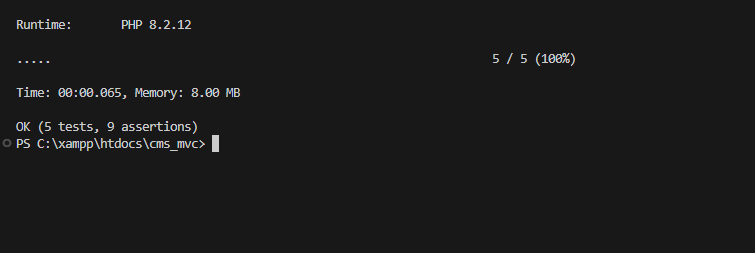
\includegraphics[width=1\linewidth]{unit1}}
	\caption{Результаты модульного тестирования}
	\label{unit1:image}
\end{figure}

\subsubsection{Системное тестирование программной системы}

Для проверки работоспособности разработанной программы было выпоненно системное тестирование. Результаты тестирования представленны в виде снимков экрана.

На рисунке \ref{ui7:image} представлена страница входа в административную панель сайта, которое открывается при запросе из адресной строки браузера. При успешной авторизации пользователь переходит на главную страницу панели и боковое меню для перемещения по соответствующим разделам панели.

\begin{figure}[H]
	\center{
\includegraphics[width=1\linewidth]{ui7}}
	\caption{Страница для входа в административную панель}
	\label{ui7:image}
\end{figure}

%Раздел "<Пользователь"> представляет функции для управления пользователями ситемы, в этом разделе отображается список пользователей \ref{main:image}, кнопки для перехода к форме добавления \ref{main:image} и редактивания \ref{main:image} пользователя.
%
%Раздел "<Страницы"> представляет функции для управления страницами сайта, в этом разделе отображается список страниц сайта \ref{main:image}, кнопки для перехода к форме добавления \ref{main:image} и редактору \ref{main:image} контента.

Для того чтобы управлять страницами сайта, пользователю необходимо перейти в раздел "<Страницы"> (рис. \ref{ui8:image}), в котором отобразиться список страниц сайта. 

\begin{figure}[H]
	\center{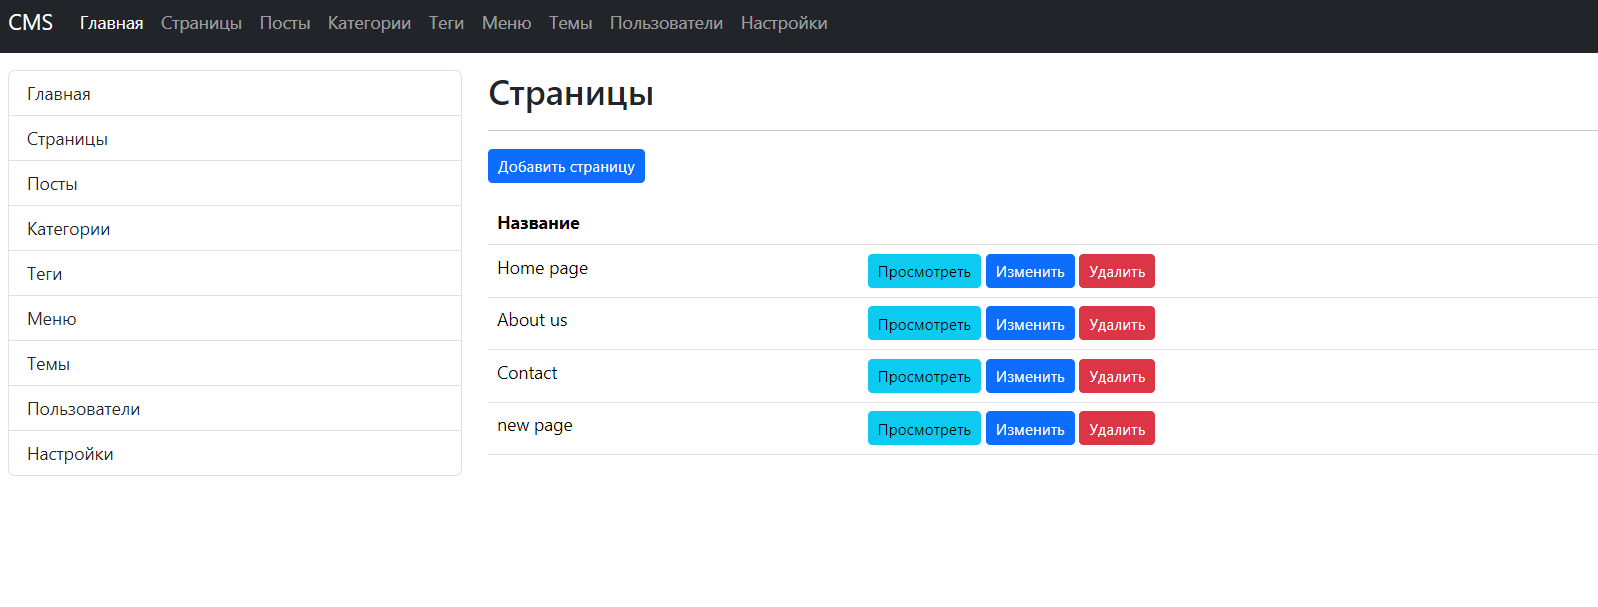
\includegraphics[width=1\linewidth]{ui8}}
	\caption{Список страниц сайта}
	\label{ui8:image}
\end{figure}

Для добавление новой страницы пользователь нажимает на кнопку "<Добавить страницу">, которая открывает форму добавления новой страницы (рис. \ref{ui9:image}). После ввода данных странцы, при нажатии на кнопку "<Добавить">, новая страница добаляется на сайт.

\begin{figure}[H]
	\center{
\includegraphics[width=1\linewidth]{ui9}}
	\caption{Форма добавления страницы}
	\label{ui9:image}
\end{figure}

Для редактирования страницы пользователь выбирает страницу из списка страниц и нажимает на кнопку "<Редактировать">, открывается редактор контента (рис. \ref{ui10:image}), в котором пользователь может вносить изменения в содержимое страницы, добавлять различные элементы интерфейса, форматировать текст и др. Для сохранения изменений пользователь нажимает на кнопку "<Сохранить">.

\begin{figure}[H]
	\center{
\includegraphics[width=1\linewidth]{ui10}}
	\caption{Редактор контента}
	\label{ui10:image}
\end{figure}

Внесенные изменения отображаюся на главной странице сайта (рис. \ref{ui11:image}).

\begin{figure}[H]
	\center{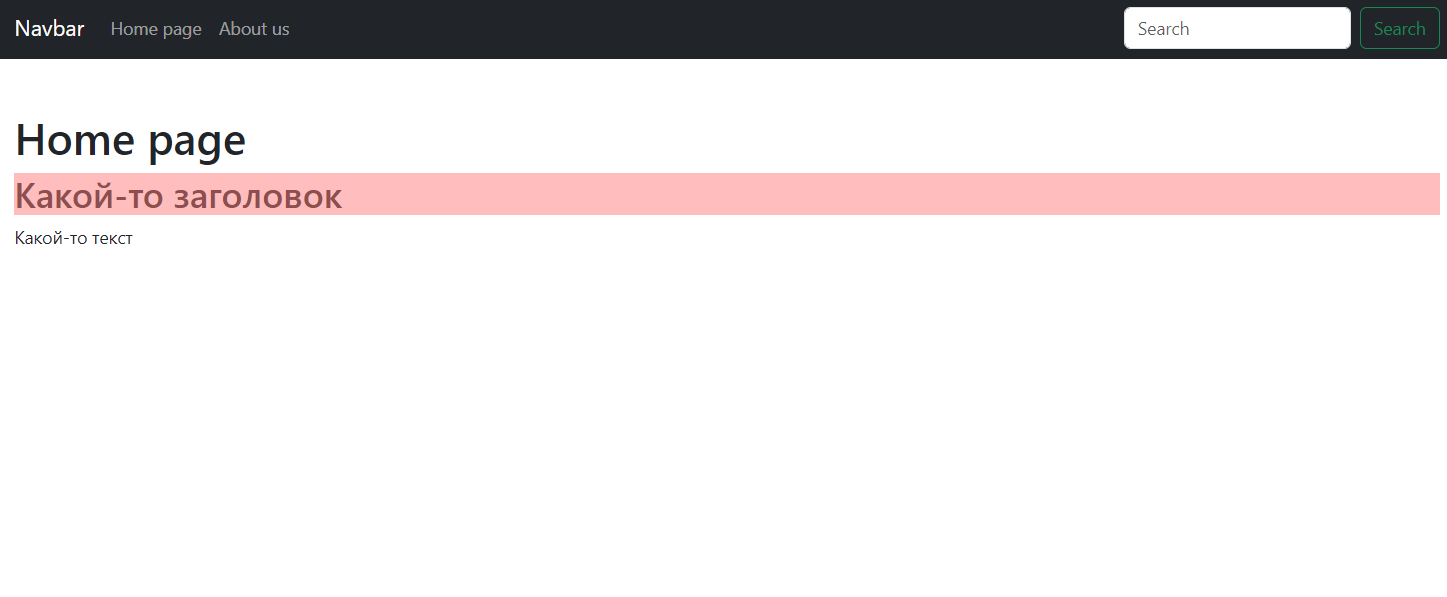
\includegraphics[width=1\linewidth]{ui11}}
	\caption{Главная страница сайта}
	\label{ui11:image}
\end{figure}

Для того чтобы управлять навигационными меню сайта, пользователю необходимо перейти в раздел "<Меню"> (рис. \ref{ui12:image}), в котором отобразиться список навигационных меню сайта.

\begin{figure}[H]
	\center{
\includegraphics[width=1\linewidth]{ui12}}
	\caption{Список областей меню сайта}
	\label{ui12:image}
\end{figure}

Для добавление нового пункта меню, пользователь выбирает область меню, открывается страница со списком пунктов меню выбранной области меню (рис. \ref{ui13:image}), пользователь нажимает на кнопку "<Добавить">, появляется выпадающий список из опций: "<Страница">, "<Произвольная ссылка">. 

\begin{figure}[H]
	\center{
\includegraphics[width=1\linewidth]{ui13}}
	\caption{Список пунктов меню}
	\label{ui13:image}
\end{figure}

После выбора одной из опций появляется форма для добавления нового пункта меню (рис. \ref{ui14:image}).

\begin{figure}[H]
	\center{
\includegraphics[width=1\linewidth]{ui14}}
	\caption{Форма добавления нового пункта меню}
	\label{ui14:image}
\end{figure}

После ввода данных пункта меню, при нажатии на кнопку "<Добавить">, новый пункт меню добавляется в меню и отображается в шапке сайта (рис. \ref{ui15:image}).

\begin{figure}[H]
	\center{
\includegraphics[width=1\linewidth]{ui15}}
	\caption{Добавленный пункт меню}
	\label{ui15:image}
\end{figure}
		
		
		
\subsection{Сборка компонентов программной системы}

Компоненты программно-информационной системы включают в себя файлы классов, скрипты, шаблоны страниц, ресурсы, библиотеки, конфигурационные файлы и прочие файлы, которые используются для функционирования системы.

Для компиляции и сборки всех программ, входящих в состав программно-информационной системы, необходимы установленный на компьютер HTTP-сервер и интерпритатор языка PHP.

Программная система запускается в браузере.

%На рисунке \ref{main:image} представлена главная страница сайта «Русатом – Аддитивные технологии».
%\newpage % при необходимости можно переносить рисунок на новую страницу
%\begin{figure}[H] % H - рисунок обязательно здесь, или переносится, оставляя пустоту
%\center{\includegraphics[width=1\linewidth]{main1}}
%\center{\includegraphics[width=1\linewidth]{main2}}
%\center{\includegraphics[width=1\linewidth]{main3}}
%\caption{Главная страница сайта «Русатом – Аддитивные технологии»}
%\label{main:image}
%\end{figure}

%На рисунке \ref{menu:image} представлен динамический вывод заголовков, включающий в себя искомые фразы при поиске фраз.

%\begin{figure}[ht]
%\center{\includegraphics[width=1\linewidth]{menu}}
%\caption{Динамический вывод заголовков}
%\label{menu:image}
%\end{figure}
%
%На рисунке \ref{enter:image} представлен ввод данных для публикации новости.
%
%\begin{figure}[ht]
%\center{\includegraphics[width=1\linewidth]{enter}}
%\caption{Ввод данных для публикации очень-очень длинной, интересной и полезной новости}
%\label{enter:image}
%\end{figure}

   \section*{ЗАКЛЮЧЕНИЕ}
\addcontentsline{toc}{section}{ЗАКЛЮЧЕНИЕ}
В процессе выполнения данной работы была создана программно-информационная система для совместного управления содержимым сайта.

Разработанная система выполняет основные функции предоставляемые большинством существующих CMS, включая управления страницами, записями (постами), управление содержимым страниц и постов, категоризацию записей, управление пользователями, выбор темы сайта, выбор шаблона отображения страниц.

Основные результаты работы:

\begin{enumerate}
\item Проведен анализ предметной области. Определены перспективы и ключевые направления разработки программной системы.
\item Разработана концептуальная модель системы. Разработана модель данных системы. Определены требования к системе.
\item Осуществлено проектирование системы. Разработана база данных. Разработана архитектура серверной части. Разработан пользовательский интерфейс административной панели системы.
\item Проведено модульное и системное тестирование программной системы.
\end{enumerate}

Все требования, объявленные в техническом задании, были полностью реализованы, все задачи, поставленные в начале разработки проекта, были также решены.

Перспективой дальнейшей разработки является расширение функционала системы: добавление новых модулей, добавления новых функций в редактор контента.
}\fi
\addcontentsline{toc}{section}{СПИСОК ИСПОЛЬЗОВАННЫХ ИСТОЧНИКОВ}

\begin{thebibliography}{20}
    \bibitem{javascript} Фримен, А. Практикум по программированию на JavaScript / А. Фримен. – Москва~: Вильямс, 2013. – 960 с. – ISBN 978-5-8459-1799-7. – Текст~: непосредственный.
   	\bibitem{uml} Фаулер, М. UML. Основы /  М. Фаулер ; пер. с англ. А. Петухова. - 3-е изд. – Санкт-Петербург~: Символ-Плюс, 2004. – 192 с. – ISBN 5-92086-060-Х. – Текст~: непосредственный
    \bibitem{php} Бретт, М. PHP и MySQL. Исчерпывающее руководство / М. Бретт. – Санкт-Петербург : Питер, 2016. – 544 с. – ISBN 978-5-496-01049-8. – Текст~: непосредственный.
    \bibitem{css} Веру, Л. Секреты CSS. Идеальные решения ежедневных задач / Л. Веру. – Санкт-Петербург : Питер, 2016. – 336 с. – ISBN 978-5-496-02082-4. – Текст~: непосредственный.
    \bibitem{mysql}	Гизберт, Д. PHP и MySQL / Д. Гизберт. – Москва~: НТ Пресс, 2013. – 320 с. – ISBN 978-5-477-01174-2. – Текст~: непосредственный.
	\bibitem{html5}	Голдстайн, А. HTML5 и CSS3 для всех / А. Голдстайн, Л. Лазарис, Э. Уэйл. – Москва~: Вильямс, 2012. – 368 с. – ISBN 978-5-699-57580-0. – Текст~: непосредственный.
	\bibitem{htmlcss} Дэкетт, Д. HTML и CSS. Разработка и создание веб-сайтов / Д. Дэкетт. – Москва~: Эксмо, 2014. – 480 с. – ISBN 978-5-699-64193-2. – Текст~: непосредственный.
	\bibitem{bigbook} Макфарланд, Д. Большая книга CSS / Д. Макфарланд. – Санкт-Петербург : Питер, 2012. – 560 с. – ISBN 978-5-496-02080-0. – Текст~: непосредственный.
	\bibitem{uchiru} Лоусон, Б. Изучаем HTML5. Библиотека специалиста / Б. Лоусон, Р. Шарп. – Санкт-Петербург : Питер, 2013 – 286 с. – ISBN 978-5-459-01156-2. – Текст~: непосредственный.
	\bibitem{chaynik} Титтел, Э. HTML5 и CSS3 для чайников / Э. Титтел, К. Минник. – Москва~: Вильямс, 2016 – 400 с. – ISBN 978-1-118-65720-1. – Текст~: непосредственный.
	\bibitem{chaynik} Ральф, Дж. Приемы объектно–ориентированного проектирования. Паттерны проектирования / Дж. Ральф, Влиссидес Джон. – СПб.: Питер, 2016. – 366 c. – ISBN 978-5-459-01720-5. – Текст~: непосредственный..
	\bibitem{metanit_php} METANIT.COM – Сайт о программировании : образовательная платформа : сайт. Санкт-Петербург, 2024. – URL: https://metanit.com/php/tutorial/ (дата обращения: 14.05.2024).
	\bibitem{metanit_js} METANIT.COM – Сайт о программировании : образовательная платформа : сайт. Санкт-Петербург, 2024. – URL: https://metanit.com/web/javascript/ (дата обращения: 14.05.2024).
	\bibitem{metanit_sql} METANIT.COM – Сайт о программировании : образовательная платформа : сайт. Санкт-Петербург, 2024. – URL: https://metanit.com/sql/tutorial/ (дата обращения: 14.05.2024).
	\bibitem{metanit_mysql}	METANIT.COM – Сайт о программировании : образовательная платформа : сайт. Санкт-Петербург, 2024. – URL: https://metanit.com/sql/mysql/ (дата обращения: 14.05.2024).
	\bibitem{metanit_query}	METANIT.COM – Сайт о программировании : образовательная платформа : сайт. Санкт-Петербург, 2024. – URL: https://metanit.com/web/jquery/ (дата обращения: 14.05.2024).
	\bibitem{metanit_html} METANIT.COM – Сайт о программировании : образовательная платформа : сайт. Санкт-Петербург, 2024. – URL: https://metanit.com/web/html5/ (дата обращения: 14.05.2024).
	\bibitem{metanit_css} METANIT.COM – Сайт о программировании : образовательная платформа : сайт. Санкт-Петербург, 2024. – URL: https://metanit.com/css/ (дата обращения: 14.05.2024).
	\bibitem{metanit_paterns} METANIT.COM – Сайт о программировании : образовательная платформа : сайт. Санкт-Петербург, 2024. – URL: https://metanit.com/paterns/ (дата обращения: 14.05.2024).	
	\bibitem{cms_dev} Developing Web Content Management Systems – from the Past to the Future : сайт. – URL: https://www.shs-conferences.org/articles/shsconf/pdf/2021/21/shsconf\_icemt2021\_05007.pdf (дата обращения: 14.05.2024).
\end{thebibliography}

\ifВКР{\appendix{Представление графического материала}

Графический материал, выполненный на отдельных листах,
изображен на рисунках А.1--А.\arabic{числоПлакатов}.
\setcounter{числоПлакатов}{0}

\renewcommand{\thefigure}{А.\arabic{figure}} % шаблон номера для плакатов

\begin{landscape}

\begin{плакат}
    
\includegraphics[width=0.82\linewidth]{плакат1.eps}
    \заголовок{Сведения о ВКРБ}
    \label{pl1:image}      
\end{плакат}

\begin{плакат}
    
\includegraphics[width=0.82\linewidth]{плакат2.eps}
    \заголовок{Цели и задачи разработки}
    \label{pl2:image}      
\end{плакат}

\begin{плакат}
    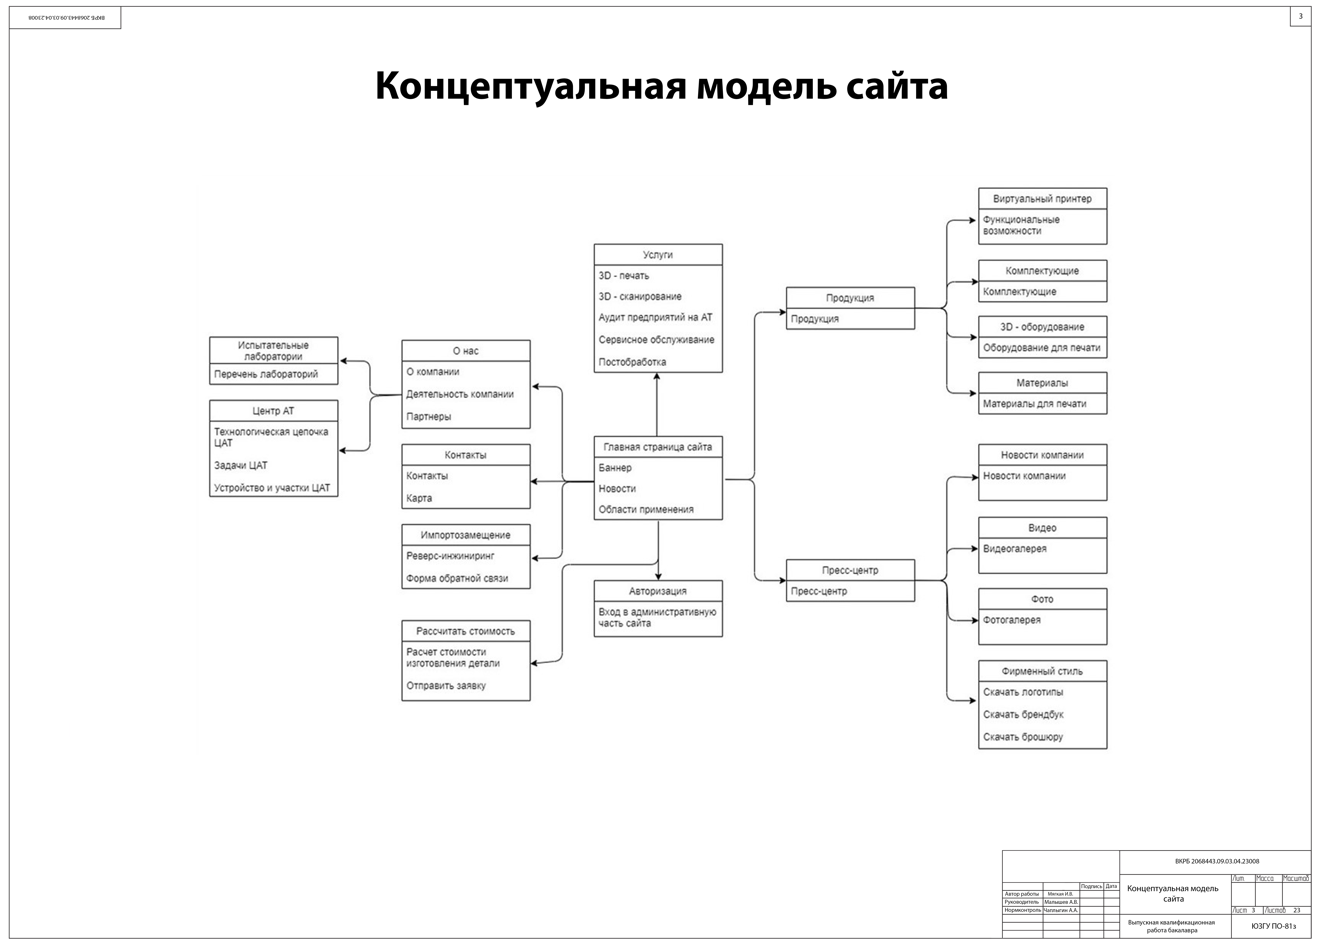
\includegraphics[width=0.82\linewidth]{плакат3.eps}
    \заголовок{Диаграмма прецедентов}
    \label{pl3:image}      
\end{плакат}

\begin{плакат}
	\includegraphics[width=0.82\linewidth]{плакат4.eps}
	\заголовок{Реляционная модель данных}
	\label{pl4:image}      
\end{плакат}

\begin{плакат}
	\includegraphics[width=0.82\linewidth]{плакат5.eps}
	\заголовок{Диаграмма компонентов}
	\label{pl5:image}      
\end{плакат}

\begin{плакат}
	\includegraphics[width=0.82\linewidth]{плакат6.eps}
	\заголовок{Диаграмма классов (часть 1)}
	\label{pl6:image}      
\end{плакат}

\begin{плакат}
	\includegraphics[width=0.82\linewidth]{плакат7.eps}
	\заголовок{Диаграмма классов (часть 2)}
	\label{pl7:image}      
\end{плакат}

\begin{плакат}
	
\includegraphics[width=0.82\linewidth]{плакат8.eps}
	\заголовок{Заключение}
	\label{pl8:image}      
\end{плакат}

\end{landscape}
}\fi
\ifПрактика{}\else{\appendix{Фрагменты исходного кода программы}

%main.tex
%\lstinputlisting[language=Tex, frame=none]{main.tex}
%
%ТехПроект.tex
%\lstinputlisting[language=Tex, frame=none]{ТехПроект.tex}

\begin{lstlisting}[language=PHP, frame=none]
<?php

namespace src;

use mysqli;

final class DatabaseConnection
{
	private static $instance = null;
	private static $connection;
	
	static function getInstance()
	{
		if (is_null(self::$instance)) {
			self::$instance = new DatabaseConnection();
		}
		return self::$instance;
	}
	
	static function connect($hostname, $user, $password, $dbName)
	{
		self::$connection = new mysqli($hostname, $user, $password, $dbName);
	}
	
	function getConnection()
	{
		return self::$connection;
	}
	
	private function __construct()
	{
	}
	
	private function __clone()
	{
	}
}

<?php

declare(strict_types=1);

namespace src;

use mysqli;

abstract class Entity
{
	public int $id;
	protected $dbConn;
	protected static string $tableName;
	protected array $fields = [];
	protected array $primaryKeys = ['id'];
	
	abstract protected function initFields(): void;
	
	protected function __construct($dbConn)
	{
		$this->dbConn = $dbConn;
		$this->initFields();
	}
	
	public static function add($dbConn, $data): static
	{
		$className = static::class;
		
		$object = new $className($dbConn);
		$object->setFieldValues((array) $data);
		$object->insert();
		
		return $object;
	}
	
	public function update(mixed $data): void
	{
		$this->setFieldValues((array) $data);
		$this->save();
	}
	
	public static function getAll($dbConn, array $conditions = []): array
	{
		return static::getObjects($dbConn, $conditions);
	}
	
	public static function getByField($dbConn, string $fieldName, $fieldValue): ?static
	{
		$objects = static::getObjects($dbConn, [$fieldName => $fieldValue]);
		return $objects[0] ?? null;
	}
	
	protected function setFieldValues(array $data): void
	{
		foreach ($this->primaryKeys as $keyName) {
			if (array_key_exists($keyName, $data)) {
				$this->$keyName = $data[$keyName];
			}
		}
		
		foreach ($this->fields as $fieldName) {
			if (array_key_exists($fieldName, $data)) {
				$this->$fieldName = $data[$fieldName];
			}
		}
	}
	
	protected function insert(): void
	{
		$parameterValues = [];
		$parameterTypes = '';
		
		foreach ($this->fields as $field) {
			$parameterValues[] = $this->$field;
			$parameterTypes .= self::getType($this->$field);
		}
		
		$fieldNames = implode(', ', $this->fields);
		$parameters = implode(', ', array_fill(0, count($this->fields), '?'));
		
		$sql = "INSERT INTO " . static::$tableName . " ($fieldNames) VALUES ($parameters)";
		
		$stmt = $this->dbConn->prepare($sql);
		$stmt->bind_param($parameterTypes, ...$parameterValues);
		$stmt->execute();
		
		$this->id = $this->dbConn->insert_id;
		
		$stmt->close();
	}
	
	protected function save(): void
	{
		$fieldBindings = [];
		$keyBindings = [];
		$parameterValues = [];
		$parameterTypes = '';
		
		foreach ($this->fields as $field) {
			$fieldBindings[] = $field . ' = ?';
			$parameterValues[] = $this->$field;
			$parameterTypes .= self::getType($this->$field);
		}
		
		foreach ($this->primaryKeys as $key) {
			$keyBindings[] = $key . ' = ?';
			$parameterValues[] = $this->$key;
			$parameterTypes .= self::getType($this->$key);
		}
		
		$fieldBindingsString = implode(', ', $fieldBindings);
		$keyBindingsString = implode(' AND ', $keyBindings);
		
		$sql = "UPDATE " . static::$tableName . " SET $fieldBindingsString WHERE $keyBindingsString";
		
		$stmt = $this->dbConn->prepare($sql);
		$stmt->bind_param($parameterTypes, ...$parameterValues);
		$stmt->execute();
		
		$stmt->close();
	}
	
	public function delete(): void
	{
		$keyBindings = [];
		$parameterValues = [];
		$parameterTypes = '';
		
		foreach ($this->primaryKeys as $key) {
			$keyBindings[] = $key . ' = ?';
			$parameterValues[] = $this->$key;
			$parameterTypes .= self::getType($this->$key);
		}
		
		$keyBindingsString = join(' AND ', $keyBindings);
		
		$sql = "DELETE FROM " . static::$tableName . " WHERE $keyBindingsString";
		
		$stmt = $this->dbConn->prepare($sql);
		$stmt->bind_param($parameterTypes, ...$parameterValues);
		$stmt->execute();
		
		$stmt->close();
	}
	
	private static function getData($dbConn, array $conditions = []): array
	{
		$sql = "SELECT * FROM " . static::$tableName;
		$fieldBindings = [];
		$types = '';
		$values = [];
		
		if ($conditions) {
			foreach ($conditions as $fieldName => $fieldValue) {
				$fieldBindings[] = "$fieldName = ?";
				$types .= self::getType($fieldValue);
				$values[] = $fieldValue;
			}
			$sql .= ' WHERE ' . implode(' AND ', $fieldBindings);
		}
		
		$stmt = $dbConn->prepare($sql);
		
		if ($conditions) {
			$stmt->bind_param($types, ...$values);
		}
		
		$stmt->execute();
		$data = $stmt->get_result()->fetch_all(MYSQLI_ASSOC);
		
		$stmt->close();
		return $data;
	}
	
	private static function getObjects($dbConn, array $conditions = []): array
	{
		$data = static::getData($dbConn, $conditions);
		$objects = [];
		
		if ($data) {
			$className = static::class;
			foreach ($data as $objectData) {
				$object = new $className($dbConn);
				$object->setFieldValues($objectData, true);
				$objects[] = $object;
			}
		}
		
		return $objects;
	}
	
	private static function getType($value): string
	{
		if (is_null($value)) {
			return 's';
		} elseif (is_int($value)) {
			return 'i';
		} elseif (is_float($value)) {
			return 'd';
		} elseif (is_string($value)) {
			return 's';
		} else {
			return 'b';
		}
	}
}

<?php

declare(strict_types=1);

namespace src;

abstract class ContentEntity extends Entity
{
	public string $title;
	public string $url;
	protected string $entityName;
	protected string $controllerName;
	protected ?string $updateAction = null;
	
	protected function initFields(): void
	{
		$this->fields = [
		'title'
		];
	}
	
	protected function setFieldValues(array $data, bool $fromDatabase = false): void
	{
		parent::setFieldValues($data);
		
		if ($fromDatabase) {
			$this->url = Route::getByField($this->dbConn, $this->entityName . '_id', $this->id)->path;
		}
	}
	
	public static function add($dbConn, $data): static
	{
		$object = parent::add($dbConn, $data);
		$object->manageRoute();
		$object->afterInsert($data);
		
		return $object;
	}
	
	public function update($data): void
	{
		parent::update($data);
		$this->manageRoute();
		$this->afterUpdate($data);
	}
	
	protected function manageRoute(): void
	{
		$this->url = $this->generateUrl();
		$route = Route::getByField($this->dbConn, $this->entityName . '_id', $this->id);
		
		if ($route) {
			$route->updatePath($this->url);
		} else {
			Route::add($this->dbConn, new RouteData($this->url, $this->controllerName, $this->entityName, $this->id, $this->updateAction));
		}
	}
	
	protected function generateUrl(): string
	{
		$url = strtolower(str_replace(' ', '-', $this->title));
		
		$parentUrl = $this->getParentUrlPath();
		if ($parentUrl) {
			$url = $parentUrl . '/' . $url;
		} else {
			$url = '/' . $this->entityName . '/' . $url;
		}
		
		return $url;
	}
	
	private function getParentUrlPath(): ?string
	{
		$parent = 'parent_' . $this->entityName . '_id';
		if (property_exists($this, $parent) && $this->$parent !== null && $this->$parent != 1) {
			return Route::getByField($this->dbConn, $this->entityName . '_id', $this->$parent)->path;
		}
		return null;
	}
	
	abstract protected function afterInsert($data): void;
	abstract protected function afterUpdate($data): void;
}

<?php

declare(strict_types=1);

namespace src;

use modules\user\admin\models\User;

class Auth
{
	function verifyLogin($dbConn, string $username, string $password): bool
	{
		$user = User::getByField($dbConn, 'username', $username);
		
		if (!$user->id) {
			return false;
		}
		if (!password_verify($password, $user->password_hash)) {
			return false;
		}
		
		$_SESSION['current_user_id'] = $user->id;
		$_SESSION['is_admin'] = $user->role == 'admin' ? true : false;
		return true;
	}
}

<?php

declare(strict_types=1);

namespace src;

class Route extends Entity
{
	protected static string $tableName = 'routes';
	public string $path;
	public string $controller;
	public ?string $action;
	public ?int $page_id = null;
	public ?int $post_id = null;
	public ?int $category_id = null;
	public ?int $tag_id = null;
	
	protected function initFields(): void
	{
		$this->fields = [
		'path',
		'controller',
		'action',
		'page_id',
		'post_id',
		'category_id',
		'tag_id'
		];
	}
	
	public static function add($dbConn, $data): static
	{
		$route = new Route($dbConn);
		$route->setFieldValues([
		'path' => $data->url,
		'controller' => $data->controller,
		$data->entity . '_id' => $data->entity_id,
		'action' => $data->action
		]);
		$route->insert();
		
		return $route;
	}
	
	public function updatePath($newPath): void
	{
		$this->path = $newPath;
		$this->save();
	}
}

<?php

namespace modules\page\models;

use modules\menu\admin\models\MenuItem;
use src\ContentEntity;
use src\Route;

class Page extends ContentEntity
{
	public function __construct($dbConn)
	{
		parent::__construct($dbConn);
	}
	
	protected static string $tableName = 'pages';
	protected string $entityName = 'page';
	protected string $controllerName = 'page';
	
	public string $content;
	public ?int $parent_page_id;
	
	protected function initFields(): void
	{
		parent::initFields();
		$this->fields[] = 'content';
		$this->fields[] = 'parent_page_id';
	}
	
	protected function afterInsert($data): void
	{
	}
	
	protected function afterUpdate($data): void
	{
		$this->updateMenuItems();
		
		$childPages = $this->getChildPages();
		foreach ($childPages as $page) {
			$page->manageRoute();
			$page->updateMenuItems();
		}
	}
	
	private function updateMenuItems(): void
	{
		$route = Route::getByField($this->dbConn, 'page_id', $this->id);
		$menuItem = MenuItem::getByField($this->dbConn, 'route_id', $route->id);
		
		if ($menuItem) {
			$menuItem->updateMenuItemUrl($this->url);
		}
	}
	
	public function getChildPages(): array
	{
		return Page::getAll($this->dbConn, ['parent_page_id' => $this->id]);
	}
}

<?php

namespace modules\post\models;

use modules\category\models\Category;
use modules\post\models\PostCategories;
use modules\user\admin\models\User;
use mysqli;
use src\ContentEntity;

class Post extends ContentEntity
{
	protected static string $tableName = 'posts';
	protected string $entityName = 'post';
	protected string $controllerName = 'post';
	
	public string $content;
	public int $author_id;
	public User $author;
	public $updated_datetime;
	public array $categories = [];
	
	protected function initFields(): void
	{
		parent::initFields();
		$this->fields = array_merge($this->fields, [
		'content',
		'author_id',
		'updated_datetime'
		]);
	}
	
	protected function setFieldValues(array $data, bool $fromDatabase = false): void
	{
		parent::setFieldValues($data, $fromDatabase);
		
		if ($fromDatabase) {
			$this->categories = $this->getCategories();
			$this->author = User::getByField($this->dbConn, 'id', $this->author_id);
		}
	}
	
	protected function afterInsert($data): void
	{
		$this->updatePostCategories($data->categories);
	}
	
	
	protected function afterUpdate($data): void
	{
		$this->updatePostCategories($data->categories);
	}
	
	private function updatePostCategories(array $categories): void
	{
		$postId = $this->id;
		$currentCategories = PostCategories::getAll($this->dbConn, ['post_id' => $postId]);
		
		foreach ($currentCategories as $category) {
			$category->delete();
		}
		
		foreach ($categories as $categoryId) {
			$data = (object)['post_id' => $postId, 'category_id' => (int)$categoryId];
			PostCategories::add($this->dbConn, $data);
		}
		
		$this->categories = $this->getCategories();
	}
	
	public function getCategories(): array
	{
		$categoryIds = $this->getCategoryIds();
		
		$categories = [];
		foreach ($categoryIds as $categoryId) {
			$category = Category::getByField($this->dbConn, 'id', $categoryId);
			$categories[] = $category;
		}
		
		return $categories;
	}
	
	public function getCategoryIds(): array
	{
		$postCategories = PostCategories::getAll($this->dbConn, ['post_id' => $this->id]);
		return array_map(fn ($postCategory) => $postCategory->category_id, $postCategories);
	}
	
	public static function getPostsByCategory(mysqli $dbConn, int $categoryId): array
	{
		$postCategories = PostCategories::getAll($dbConn, ['category_id' => $categoryId]);
		$postIds = array_map(fn ($postCategory) => $postCategory->post_id, $postCategories);
		
		$posts = [];
		foreach ($postIds as $postId) {
			$post = Post::getByField($dbConn, 'id', $postId);
			$posts[] = $post;
		}
		
		return $posts;
	}
}

<?php

namespace modules\menu\admin\models;

use src\Entity;

class Menu extends Entity
{
	protected static string $tableName = 'menus';
	public string $name;
	
	protected function initFields(): void
	{
		$this->fields = [
		'name'
		];
	}
	
	public function getMenuItems(): array
	{
		$menuItems = MenuItem::getAll($this->dbConn, ['menu_id' => $this->id]);
		
		usort($menuItems, fn($a, $b) => $a->order_num <=> $b->order_num);
		
		return $menuItems;
	}
	
	public function getAddedPageIds(): array
	{
		$sql = "SELECT page_id FROM routes INNER JOIN menu_items ON menu_items.route_id=routes.id WHERE menu_items.menu_id=?";
		// $sql = "SELECT page_id FROM routes INNER JOIN menu_items ON menu_items.url=routes.path WHERE menu_items.menu_id=$menu_id";
		$stmt = $this->dbConn->prepare($sql);
		$stmt->bind_param('i', $this->id);
		$stmt->execute();
		$result = $stmt->get_result();
		
		$addedPageIds = [];
		while ($row = $result->fetch_assoc()) {
			$addedPageIds[] = $row['page_id'];
		}
		
		return $addedPageIds;
	}
	
	private function getNextOrderNum(): int
	{
		$sql = "SELECT MAX(order_num) AS max_order_num FROM menu_items WHERE menu_id=?";
		$stmt = $this->dbConn->prepare($sql);
		$stmt->bind_param('i', $this->id);
		$stmt->execute();
		$result = $stmt->get_result();
		$row = $result->fetch_assoc();
		
		$maxOrderNum = $row['max_order_num'];
		
		return $maxOrderNum !== null ? $maxOrderNum + 1 : 1;
	}
	
	public function addMenuItem(MenuItemData $data) : MenuItem
	{
		$menuItem = new MenuItem($this->dbConn);
		
		$menuItem->setFieldValues([
		'menu_id' => $this->id,
		'title' => $data->title,
		'url' => $data->url,
		'order_num' => $this->getNextOrderNum(),
		'route_id' => $data->route_id,
		'parent_menu_item_id' => $data->parent_menu_item_id
		]);
		$menuItem->insert();
		
		return $menuItem;
	}
	
	public function updateMenuItemsOrder($newOrder)
	{
		foreach ($newOrder as $index => $itemId) {
			$itemId = (int)$itemId;
			$menu_item = MenuItem::getByField($this->dbConn, 'id', $itemId);
			$menu_item->setFieldValues(['order_num' => $index + 1]);
			$menu_item->save();
		}
	}
}

<?php

namespace modules\menu\admin\models;

use src\Entity;

class MenuItem extends Entity
{
	protected static string $tableName = 'menu_items';
	public int $menu_id;
	public string $title;
	public string $url;
	public ?int $parent_menu_item_id;
	public ?int $route_id;
	public int $order_num;
	public array $child_menu_items = [];
	
	protected function initFields(): void
	{
		$this->fields = [
		'menu_id',
		'title',
		'url',
		'parent_menu_item_id',
		'route_id',
		'order_num'
		];
	}
	
	protected function setFieldValues(array $data, bool $fromDatabase = false): void
	{
		parent::setFieldValues($data);
		
		if ($fromDatabase) {
			$this->child_menu_items = $this->getChildMenuItems();
		}
	}
	
	public function getChildMenuItems(): array
	{
		return MenuItem::getAll($this->dbConn, ['parent_menu_item_id' => $this->id]);
	}
	
	public function renderMenuItem()
	{
		$html = '<li class="list-group-item" id="' . $this->id . '">';
		$html .= $this->title;
		$html .= ' <a href="/admin/index.php?module=menu&action=editMenuItem&id=' . $this->id . '">Изменить</a> ';
		$html .= ' <a href="/admin/index.php?module=menu&action=deleteMenuItem&id=' . $this->id . '">Удалить</a> ';
		
		if (!empty($this->child_menu_items)) {
			
			$html .= '<button class="btn btn-sm btn-primary float-end" data-bs-toggle="collapse" data-bs-target="#submenu' . $this->id . '">Подробнее</button>';
			$html .= '<ul class="menu-list list-group collapse" id="submenu' . $this->id . '">';
			
			foreach ($this->child_menu_items as $child) {
				$html .= $child->renderMenuItem();
			}
			$html .= '</ul>';
		}
		$html .= '</li>';
		
		return $html;
	}
	
	public function update($data): void
	{
		$this->setFieldValues([
		'title' => $data->title,
		'url' => $data->url,
		'parent_menu_item_id' => $data->parent_menu_item_id,
		'route_id' => $data->route_id
		]);
		$this->save();
	}
	
	public function updateMenuItemUrl(string $url): void
	{
		$this->url = $url;
		$this->save();
	}
}

<?php

namespace modules\category\models;

use src\ContentEntity;

class Category extends ContentEntity
{
	protected static string $tableName = 'categories';
	protected string $entityName = 'category';
	protected string $controllerName = 'post';
	protected ?string $updateAction = 'showByCategory';
	
	public ?int $parent_category_id;
	
	protected function initFields(): void
	{
		parent::initFields();
		$this->fields[] = 'parent_category_id';
	}
	
	protected function afterInsert($data): void
	{
	}
	
	protected function afterUpdate($data): void
	{
		$childCategories = $this->getChildCategories();
		foreach ($childCategories as $category) {
			$category->manageRoute();
		}
	}
	
	public function getChildCategories(): array
	{
		return Category::getAll($this->dbConn, ['parent_category_id' => $this->id]);
	}
}

<?php

namespace modules\dashboard\admin\controllers;

use src\Controller;
use src\Auth;

class DashboardController extends Controller
{
	function defaultAction()
	{
		header('Location: /admin/index.php?module=page');
		exit();
	}
	
	function loginAction()
	{
		if ($_POST['postAction'] ?? 0) {
			$username = $_POST['username'] ?? '';
			$password = $_POST['password'] ?? '';
			
			$auth = new Auth();
			if ($auth->verifyLogin($this->dbConn, $username, $password)) {
				$_SESSION['logged_in'] = true;
				header('Location: /admin/');
				exit();
			}
			// var_dump($password);
			$_SESSION['validation']['error'] = "Username or password is incorrect";
		}
		
		include VIEW_PATH . 'admin/login.php';
		unset($_SESSION['validation']['error']);
	}
}

<?php

declare(strict_types=1);

namespace modules\page\admin\controllers;

use modules\page\models\PageData;
use src\AdminController;
use modules\page\models\Page;

class PageController extends AdminController
{
	function defaultAction(): void
	{
		$data['pages'] = Page::getAll($this->dbConn);
		
		$this->template->renderView($data, 'page/admin/views/page_list');
	}
	
	function editPageAction(): void
	{
		$pageId = $_GET['id'];
		$page = Page::getByField($this->dbConn, 'id', $pageId);
		
		if ($_POST['action'] ?? 0) {
			$page->update(new PageData(
			$_POST['title'],
			$_POST['content'],
			(int)$_POST['parent_page_id']
			));
		}
		
		$data['page'] = $page;
		$data['pages'] = Page::getAll($this->dbConn);
		$data['child_pages'] = $page->getChildPages();
		
		$pages = Page::getAll($this->dbConn);
		$child_pages = $page->getChildPages();
		// $this->template->renderView($data, 'page/admin/views/page_edit');
		include VIEW_PATH . 'admin/content_editor.php';
	}
	
	function addPageAction(): void
	{
		if ($_POST['action'] ?? 0) {
			Page::add($this->dbConn, new PageData(
			$_POST['title'],
			$_POST['content'],
			(int)$_POST['parent_page_id']
			));
			
			header('Location: /admin/');
			exit();
		}
		
		$data['pages'] = Page::getAll($this->dbConn);
		$this->template->renderView($data, 'page/admin/views/page_add');
	}
	
	function deletePageAction(): void
	{
		$pageId = $_GET['id'];
		$page = Page::getByField($this->dbConn, 'id', $pageId);
		$page->delete();
		
		header('Location: /admin/');
	}
}

<?php

namespace modules\post\admin\controllers;

use modules\category\models\Category;
use modules\post\models\PostData;
use src\AdminController;
use modules\post\models\Post;

class PostController extends AdminController
{
	function defaultAction(): void
	{
		$data['posts'] = Post::getAll($this->dbConn);
		
		$this->template->renderView($data, 'post/admin/views/post_list');
	}
	
	function addPostAction(): void
	{
		if ($_POST['action'] ?? 0 == 1) {
			Post::add($this->dbConn, new PostData(
			$_POST['title'],
			$_POST['content'],
			$_SESSION['current_user_id'],
			$_POST['categories'] ?? [1]
			));
			
			header('Location: /admin/index.php?module=post');
			exit();
		}
		
		$categories = Category::getAll($this->dbConn);
		array_shift($categories);
		
		$data['categories'] = $categories;
		$this->template->renderView($data, 'post/admin/views/post_add');
	}
	
	function editPostAction(): void
	{
		$postId = $_GET['id'];
		$post = Post::getByField($this->dbConn, 'id', $postId);
		
		if ($_POST['action'] ?? 0) {
			$post->update(new PostData(
			$_POST['title'],
			$_POST['content'],
			$_SESSION['current_user_id'],
			$_POST['categories'] ?? [1]
			));
		}
		
		$data['post'] = $post;
		$data['post_categories'] = $post->getCategoryIds();
		
		$categories = Category::getAll($this->dbConn);
		array_shift($categories);
		
		$data['categories'] = $categories;
		// $page = $pageObj;
		// $pages = $pageObj->getAll();
		// $child_pages = $pageObj->getChildPages();
		$this->template->renderView($data, 'post/admin/views/post_edit');
		// include VIEW_PATH . 'admin/content_editor.php';
	}
	
	function deletePostAction(): void
	{
		$postId = $_GET['id'];
		$postObj = Post::getByField($this->dbConn, 'id', $postId);
		$postObj->delete();
		
		header('Location: /admin/index.php?module=post');
	}
}

<?php

declare(strict_types=1);

namespace modules\menu\admin\controllers;

use modules\menu\admin\models\Menu;
use src\AdminController;;
use modules\menu\admin\models\MenuItem;
use modules\menu\admin\models\MenuItemData;
use modules\page\models\Page;
use src\Route;

class MenuController extends AdminController
{
	function defaultAction(): void
	{
		$data['menus'] = Menu::getAll($this->dbConn);
		
		$this->template->renderView($data, 'menu/admin/views/menu_list');
	}
	
	function editMenuAction(): void
	{
		$menuId = $_GET['id'];
		
		$menu = Menu::getByField($this->dbConn, 'id', $menuId);
		
		$data['menu'] = $menu;
		$data['menu_items'] = $menu->getMenuItems();
		
		$this->template->renderView($data, 'menu/admin/views/menu_edit');
	}
	
	function editMenuItemAction(): void
	{
		$menuItemId = $_GET['id'];
		
		$menuItem = MenuItem::getByField($this->dbConn, 'id', $menuItemId);
		
		if ($_POST['action'] ?? 0) {
			
			$parentMenuItemId = (int)$_POST['parent_menu_item_id'];
			if ($parentMenuItemId === 0) {
				$parentMenuItemId = null;
			}
			$menuItem->update(new MenuItemData($_POST['title'], $menuItem->url, $parentMenuItemId));
		}
		
		$data['menu_item'] = $menuItem;
		$data['menu_items'] = MenuItem::getAll($this->dbConn, ['menu_id' => $menuItem->menu_id]);
		
		$this->template->renderView($data, 'menu/admin/views/menu_item_edit');
	}
	
	function addMenuItemAction(): void
	{
		$menuId = $_GET['id'];
		
		$menu = Menu::getByField($this->dbConn, 'id', $menuId);
		
		if ($_POST['action'] ?? 0) {
			
			if ($_GET['type'] == 'page') {
				foreach ($_POST['page_ids'] as $pageId) {
					$page = Page::getByField($this->dbConn, 'id', $pageId);
					$route = Route::getByField($this->dbConn, 'page_id', $pageId);
					
					$menu->addMenuItem(new MenuItemData(
					$page->title,
					$page->url,
					route_id: $route->id
					));
				}
			} else if ($_GET['type'] == 'link') {
				$parentMenuItemId = (int)$_POST['parent_menu_item_id'];
				if ($parentMenuItemId === 0) {
					$parentMenuItemId = null;
				}
				$menu->addMenuItem(new MenuItemData(
				$_POST['title'],
				$_POST['url'],
				$parentMenuItemId
				));
			}
			header("Location: /admin/index.php?module=menu&action=editMenu&id=$menuId");
			exit();
		}
		
		$data['pages'] = Page::getAll($this->dbConn);
		$data['menu_items'] = $menu->getMenuItems();
		$data['added_page_ids'] = $menu->getAddedPageIds();
		
		if ($_GET['type'] == 'page') {
			$this->template->renderView($data, 'menu/admin/views/menu_item_add_page');
		} else if ($_GET['type'] == 'link') {
			$this->template->renderView($data, 'menu/admin/views/menu_item_add');
		}
	}
	
	function deleteMenuItemAction(): void
	{
		$menuItemId = $_GET['id'];
		$menuItem = MenuItem::getByField($this->dbConn, 'id', $menuItemId);
		$menuItem->delete();
		
		header("Location: /admin/index.php?module=menu&action=editMenu&id=$menuItem->menu_id");
	}
	
	function updateMenuOrderAction(): void
	{
		$newOrder = $_POST['order'];
		$menu = new Menu($this->dbConn);
		$menu->updateMenuItemsOrder($newOrder);
	}
}

<?php

namespace modules\category\admin\controllers;

use modules\category\models\Category;
use modules\category\models\CategoryData;
use src\AdminController;

class CategoryController extends AdminController
{
	function defaultAction(): void
	{
		$categories = Category::getAll($this->dbConn);
		array_shift($categories);
		$data['categories'] = $categories;
		
		$this->template->renderView($data, 'category/admin/views/category_list');
	}
	
	function editCategoryAction(): void
	{
		$categoryId = $_GET['id'];
		$category = Category::getByField($this->dbConn, 'id', $categoryId);
		
		if ($_POST['action'] ?? 0) {
			
			if (empty($_POST['parent_category_id'])) {
				unset($_POST['parent_category_id']);
			}
			
			$category->update(new CategoryData(
			$_POST['title'],
			$_POST['parent_category_id'] ?? null
			));
		}
		
		$data['category'] = $category;
		$data['child_categories'] = $category->getChildCategories();
		$categories = Category::getAll($this->dbConn);
		array_shift($categories);
		$data['categories'] = $categories;
		$this->template->renderView($data, 'category/admin/views/category_edit');
	}
	
	function addCategoryAction(): void
	{
		if ($_POST['action'] ?? 0) {
			
			if (empty($_POST['parent_category_id'])) {
				unset($_POST['parent_category_id']);
			}
			
			Category::add($this->dbConn, new CategoryData(
			$_POST['title'],
			$_POST['parent_category_id'] ?? null
			));
			
			header('Location: /admin/index.php?module=category');
			exit();
		}
		
		$categories = Category::getAll($this->dbConn);
		array_shift($categories);
		$data['categories'] = $categories;
		$this->template->renderView($data, 'category/admin/views/category_add');
	}
	
	function deleteCategoryAction(): void
	{
		$categoryId = $_GET['id'];
		$category = Category::getByField($this->dbConn, 'id', $categoryId);
		$category->delete();
		
		header('Location: /admin/index.php?module=category');
	}
}

<?php

declare(strict_types=1);
namespace src;

use modules\menu\admin\models\Menu;
use modules\menu\admin\models\MenuItem;
use mysqli;

class Template
{
	private string $templatePath;
	private string $context;
	private mysqli $dbConn;
	
	function __construct(mysqli $dbConn, string $templatePath, string $context = 'site')
	{
		$this->dbConn = $dbConn;
		$this->templatePath = $templatePath;
		$this->context = $context;
	}
	
	function renderView(array $data, ?string $view = null, ?string $selected_theme = null) : void
	{
		extract($data);
		
		
		if ($this->context === 'admin'){
			include VIEW_PATH . $this->templatePath . ".php";
		}
		else{
			$menus = Menu::getAll($dbConn);
			// $index = array_search('header_menu', array_column($menus, 'name'));
			// $headerMenu = $index !== false ? $menus[$index] : null;
			include THEMES_PATH . $selected_theme . '/' . $this->templatePath . ".php";
		}
	}
}

	
\end{lstlisting}

\ifВКР{
\newpage
\addcontentsline{toc}{section}{На отдельных листах (CD-RW в прикрепленном конверте)}
\begin{center}
\textbf{Место для диска}
\end{center}
}\fi
}\fi
\end{document}
